\documentclass[12pt, letterpaper]{article}
\usepackage[letterpaper, margin = 2.54cm]{geometry}

% dependencies

\usepackage[round]{natbib}
\usepackage[utf8]{inputenc} 
\usepackage[T1]{fontenc}
\usepackage[french]{babel}
\usepackage{geometry}
\usepackage[table]{xcolor}
\usepackage{setspace}
\usepackage[hidelinks]{hyperref}
\hypersetup{
    colorlinks=true,
    linkcolor=black,
    citecolor=blue,
    urlcolor=blue
}
\usepackage{graphicx}
\usepackage{booktabs}
\usepackage{amsmath}
\usepackage{float}
\usepackage{xcolor}


% change to nicer bullets
\renewcommand{\FrenchLabelItem}{\textbullet}

% change to Tableau instead of Table for table captions in French
\addto\captionsfrench{\def\tablename{Tableau}}


\title{\Large\textbf{Évaluation des critères permettant d'améliorer\\
l'efficacité des passages fauniques adaptés aux\\
amphibiens et reptiles\\[2em]
Projet R875.1}\\[2em]
\Large Rapport d'avancement 3}

\author{
Robin Besançon, M. Sc.\\
Professionnel de recherche\\[1em]
Aurore Fayard, M.Sc\\
Professionnelle de recherche\\[1em]
Marc J. Mazerolle, Ph.D\\
Chercheur principal}

\date{
\vspace{1em}
Réalisé pour le compte du ministère des Transports et de la Mobilité Durable\\[2em]
Juillet 2025
}




%%%%%%%%%% the following macros are necessary to track changes in document
%%%%%%%%%%%%%%%%BEGIN code added to track changes%%%%%%%%%%%%%%%%%%
\usepackage[utf8]{inputenc}

\usepackage{soulutf8}
\usepackage[normalem]{ulem}
%adding comments in margins
\usepackage[textwidth=2cm, colorinlistoftodos]{todonotes}

% just adding text in blue
\newcommand{\add}{\textcolor{blue}}

% adding and underlining text - MJM in blue
\newcommand{\addM}{\textcolor{blue}{\bgroup}\markoverwith{\textcolor{blue}{\rule[-0.5ex]{2pt}{0.4pt}}}\ULon}

% deleting text and underlining - MJM in red
\newcommand\delM{\textcolor{red}{\bgroup}\markoverwith{\textcolor{red}{\rule[0.5ex]{2pt}{0.4pt}}}\ULon}

% deleting text - MJM in red
\newcommand\underM{\textcolor{red}{\bgroup}\markoverwith{\textcolor{red}{\rule[-0.5ex]{2pt}{0.4pt}}}\ULon}


%modify color, add counter, author name, and size - MJM in blue
\newcounter{todocounter}
\newcommand{\comM}[2][]
{\stepcounter{todocounter}\todo[color=orange, size=\footnotesize, author=MJM, #1]{\thetodocounter: #2}}

%%%%%%%%%%%%%%%%END code added to track changes%%%%%%%%%%%%%%%%%%%modify color


\begin{document}

\maketitle
\vfill
\noindent

\includegraphics[width=4cm]{logos/logo_ulaval.pdf}\hfill
\includegraphics[width=4cm]{logos/logo_mtmd.png}

\pagenumbering{gobble} 

\newpage
\pagenumbering{roman}

La présente étude a été réalisée à la demande du ministère des Transports et de la Mobilité durable du Québec (MTMD). Le projet a été financé par le ministère. 
Les opinions exprimées dans le présent rapport n’engagent que la responsabilité de leurs auteurs et ne reflètent pas nécessairement les positions du ministère des Transports et de la Mobilité durable.

\vfill
\noindent
\copyright\ Université Laval, 2026
\section*{Comité de suivi}

\begin{itemize}
\item Marc J. Mazerolle (chercheur principal), Professeur titulaire et chercheur en biologie de la conservation, Département des sciences du bois et de la forêt, Université Laval.
\item Aurore Fayard, Professionnelle de recherche, laboratoire Mazerolle, Université Laval.
\item Robin Besançon, Professionnel de recherche, laboratoire Mazerolle, Université Laval.
\item Emmanuelle Viau, biologiste, chargée de projet, MTMD.
\item Marie-Michèle Ouellet-Bernier en remplacement de Coumba Cissé, conseillère à la recherche, Direction de la coordination de la recherche et de l'innovation, MTMD.
\item Mélanie Goulet, technicienne en géomatique et bioécologie, DGPRMM, MTMD.
\item Pierluc Marcoux-Viel, biologiste, Direction générale de l'Estrie, MTMD.
\item Josée Emond, ingénieure en hydraulique, Direction générale des structures, MTMD.
\item Julie Boucher, biologiste, Direction de l'environnement, MTMD.
\item Jean-Bastien Denis, ingénieur en drainage et mandats spéciaux, Direction générale de l'exploitation du réseau métropolitain, MTMD.
\item Lyne Bouthillier, biologiste, experte de la Rainette faux-grillon de l'Ouest, MELCCFP.
\item Marc-André Bouchard, aménagiste du territoire, chef d'équipe en aménagement et développement, Direction des aires protégées, MELCCFP.
\item Pierre-André Bernier, biologiste, Unité du rétablissement des espèces en péril, Service canadien de la faune, Environnement et Changement climatique Canada.
\item Vanessa Charbonneau, biologiste, chargée de projets Acquisition, gestion et mise en valeur, Nature-Action Québec.
\end{itemize}


\section*{Groupe de spécialistes}

\begin{itemize}
\item Julie Munger, botaniste, DGPRMM, MTMD.
\item Thérèse Fortin, ingénieure en électrotechnique, DGPRMM, MTMD.
\item Étienne Drouin, biologiste, Direction générale de la Faune Estrie-Montréal-Montérégie-Laval (DGFEMML), MELCCFP.
\item Elisabeth Correia Morreau, M. Sc. Biologiste, chargée de projet, direction de l'évaluation environnementale des projets terrestres, MELCCFP.
\item Alexandre Skeates, biologiste, Ville de Brossard.
\item Patrick Galois, biologiste, Amphibia Nature.
\item Patrick Paré, biologiste, directeur de la conservation et de la recherche, Zoo de Granby.
\end{itemize}


\tableofcontents
\newpage

\listoftables


\newpage
\listoffigures
\newpage

L'équipe de recherche de l'Université Laval est chargée de documenter les critères permettant d'améliorer l'efficacité des passages fauniques adaptés aux amphibiens et reptiles, ci-après appelé "le projet" pour faciliter la lecture. Nous agissons sous le financement du Contrat de recherche R875.1 entre le ministère des Transports et de la Mobilité durable (MTMD) et l'Université Laval, signé le 6 juin 2023. Un avenant au contrat de recherche a été signé le 21 mai 2025.

\pagenumbering{arabic}

\part{Passages fauniques potentiels avant travaux}


\section{Mise en contexte}

\subsection{Introduction}

Les routes réduisent la continuité écologique des milieux et constituent un obstacle physique et biologique à la faune et à la flore \citep{forman1998}. Lorsqu'une route est créée, cette nouvelle barrière peut réduire l'abondance d'une population en augmentant la mortalité \citep{seiler2020,rytwinski2016}. Plusieurs milliards d'animaux sont tués annuellement sur les routes, et la majorité des études ciblent sur les carnivores et les ongulés \citep{barrientos2021}. Pourtant, la traversée des routes est d'autant plus dangereuse pour la faune qui n'a pas une grande capacité de déplacement, et qui emprunte le même chemin pour rejoindre différents habitats chaque année \citep{gunson2019, jones2022, langen2009}. À long terme, cette fragmentation due aux routes affectera le maintien de certaines populations animales et végétales \citep{gonzalezgallina2013}.  
Au Canada, peu de passages fauniques sont spécifiquement conçus pour l'herpétofaune. Les rares projets de recherche sur ces taxons ont été réalisés sur des routes secondaires avec des passages de petits diamètres \citep{retamal2020}, ce qui n'est pas représentatif du paysage routier global. Pourtant, de nombreuses espèces souffrent d'une perte de connectivité imputable à la fragmentation du paysage, en partie lié à la multiplication des routes. C'est le cas de la rainette faux-grillon (Pseudacris triseriata) de la région de la Montérégie au Québec, qui a été désignée menacée selon la Loi sur les espèces en péril du Canada \citep{cosepac2008} et la Loi sur les espèces menacées ou vulnérables (L.R.Q., c. E-12.01). La tortue serpentine (Chelydra serpentina), tout comme la tortue peinte du Centre (Chrysemys picta marginata) et la tortue peinte de l’Est (Chrysemys picta picta) sont désignées par la Loi sur les espèces en péril du Canada comme espèces préoccupantes à l’Annexe 1.
L'objectif de ce projet vise à combler les lacunes sur les critères favorisant la connectivité écologique de la petite faune. Les résultats de ces travaux de recherche serviront à la planification d'autres projets à long terme, appliquant la méthodologie Before-After Control-Impact (BACI) aux passages adaptés à l'herpétofaune \citep{jones2022}.

\subsection{Changement d'orientation du projet de recherche}

Un premier livrable du projet de recherche R875.1 a été remis en juin 2024. Durant la rencontre de suivi 1 en septembre 2024, le ministère des Transports et de la Mobilité durable (MTMD) a annoncé que le calendrier des aménagements de passages fauniques sur l’Autoroute 10 (A10) et la Route 104 (R104) étaient reportés sans date fixe pour la prévision des travaux sur ces deux axes routiers. Les travaux du MTMD devaient consister à : (1) élargir les chaussées afin de fluidifier le trafic et de réduire la congestion automobile aux heures de pointe, tout en encourageant l’utilisation des transports en commun et le covoiturage; (2) remplacer et modifier certains ponceaux pour les aménager en passages fauniques spécifiques à l’herpétofaune. L'équipe du laboratoire de recherche en biologie de la conservation quantitative de l'Université Laval a été mandatée pour inventorier et suivre l'herpétofaune en amont et en aval des travaux. En l’absence de date prévue pour la construction des passages fauniques sur l’A10 et la R104, l’équipe de recherche a proposé un avenant au projet afin de réorienter les objectifs initiaux en fonction de ces nouvelles contraintes. Cet avenant a été approuvé par l’ensemble des parties le 21 mai 2025. Le budget du projet de recherche est inchangé, seuls les objectifs ont été modifiés. 

\begin{figure}[H]
\centering
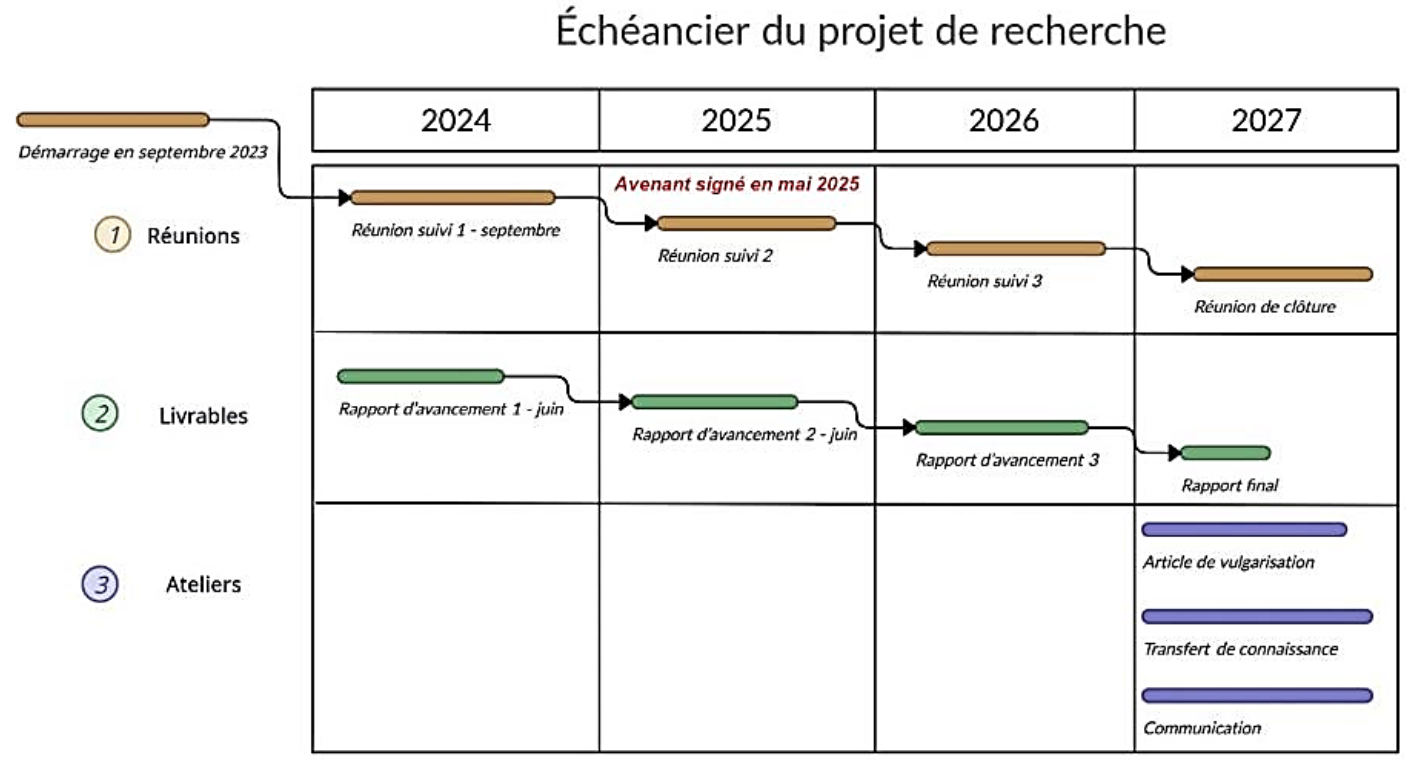
\includegraphics[width=0.8\textwidth]{figs_monteregie_liv3/echeancier.png}
\caption{Échéancier du projet de recherche entre 2023 et 2027. L'avenant 1 du
contrat R875.1 a été signé en mai 2025.}
\label{fig:echeancier26}
\end{figure}

Suite à ces changements, le deuxième livrable fut compartimenté en deux parties. Une partie était dédiée aux passages fauniques sur l'A10 et la 104. Une deuxième partie était dédiée à l'évaluation des critères de connectivité écologique. Par conséquent, le troisième et quatrième livrables suivront la même trâme afin de rendre compte des différents volets.

Dans ce troisième livrable, nous présentons les dernières avancées en matière d'échantillonnage et d'analyse des fichiers numériques, soit les images des pièges photographiques et les enregistrements des Audiomoths. Bien que nous y dressions un portrait détaillé des résultats obtenus à ce jour, ce rapport ne comporte pas d'analyses statistiques avancées. Celles-ci seront présentées dans le dernier livrable, une fois la compilation des derniers résultats finalisée pour 2026 et les derniers fichiers numériques analysés.

Nous ne reviendrons pas sur les résultats de terrain de 2024, déjà traités dans le livrable précédent. Dans la partie II, nous exposons les résultats issus de l'analyse par MegaDetector de l'ensemble des images captées par les pièges photographiques installés sur l'A10 et la 104 en 2024. Nous présentons ensuite les derniers résultats obtenus en 2025 pour les suivis de mortalité ainsi que pour les inventaires des milieux humides et de la petite faune, auxquels s'ajoutent les analyses des images des pièges photographiques déployés dans 18 ponceaux en 2025, soit 54\% des images récoltées cette année-là. L'échéancier présenté à la Fig.~\ref{fig:echeancier26} illustre les prochaines étapes du projet. 

À la suite de chaque dépôt de rapport, le comité aura l’occasion de lire et de commenter le document. Le comité de suivi se réunira pour une présentation du présent rapport par l'équipe de recherche, et les membres du comité pourront fournir des commentaires, demander des précisions, ou formuler des recommandations pour la suite. Enfin, une fois le rapport final du projet déposé et la réunion de clôture terminée, une activité de transfert technologique pourra être proposée sous forme d'atelier ou de colloque en invitant différents partenaires des milieux municipaux, gouvernementaux et académiques.





\section{Méthodes}
  
\subsection{Mortalité routière}

\subsubsection{Détection de carcasses à pied et à partir d'un véhicule}

Nous avons comparé les détections de carcasses et d'individus vivants de tous les taxons \addM{vertébrés} (amphibiens, reptiles, mammifères, oiseaux) sur la chaussée de l'A10 et de la R104 en utilisant le suivi à pied par jumelles\delM{,} et le suivi par enregistrement avec caméra GoPro fixée sur un véhicule. Lors de l'échantillonnage sur l'A10, la voie Sud était séparée de la voie Nord afin de réaliser deux décomptes indépendants.Lors de ces périodes d'enregistrement, les observateurs ne notaient pas \comM[inline]{Je ne comprends pas ce que tu veux dire par les carcasses en parallèle. Clarifier.}d'observations de carcasses en parallèle pour des raisons de sécurité. Lors d'une même journée d'échantillonnage, le même segment de route était parcouru à l'aide des deux méthodes : suivi à pied par jumelles \delM{entre 15 et 30 m de la chaussée} et enregistrement par caméra GoPro fixée sur un véhicule circulant sur la chaussée. Afin de réduire la probabilité de retrait des carcasses sur la route par des prédateurs ou des automobiles, ces suivis étaient effectués dès le lever du soleil. Lors d'une journée donnée, nous avons déterminé aléatoirement l’ordre des méthodes utilisées \addM{pour un même tronçon}. Le but était de comparer l'efficacité des deux méthodes à détecter sur la route les mêmes carcasses et les mêmes individus vivants. Il était donc important de réaliser les deux suivis dans un court laps de temps (même matinée) \addM{sur le même tronçon}. L’utilisation des deux méthodes permettra de mieux estimer le nombre réel de carcasses sur la route.

Le suivi par jumelles consistait à parcourir à pied les sentiers situés à proximité des tronçons de l'A10 et de la R104, en restant entre 15 et 30 m de la chaussée. Au moins deux observateurs réalisaient l'inventaire. Le port d'un gilet de sécurité réfléchissant et d'un casque était obligatoire en tout temps pour augmenter la visibilité du personnel sur le terrain. Les jumelles utilisées étaient des Nikon Prostaff P3 8X42 (Nikon, Tokyo, Japon). Toutes les carcasses observées sur les routes étaient géolocalisées à l'aide d'un GPS GARMIN GPSMAP 79s (Garmin, Schaffhausen, Suisse). Le suivi par caméra réalisé par voiture utilisait une caméra GoPro Hero Black 11 (GoPro, San Mateo, Californie, États-Unis) afin d'enregistrer les images sur la chaussée avec une qualité 4K, un ratio 4:3 et 30 images par seconde. Lors d'une session d'échantillonnage, la caméra GoPro était insérée dans un étui imperméable transparent et fixée à un trépied magnétique (3-Footed Monster, Sydney, Australie). Le trépied magnétique était fixé au milieu du capot avant de la voiture. La caméra pouvait être contrôlée à distance par protocole Bluetooth à l'aide de l'application gratuite Quik pour Android. Nous lancions l'enregistrement lorsque le véhicule entrait dans le segment suivi jusqu'à la fin du parcours. Les fichiers vidéo ont été visionnés et les données d'observation sur la route ont été saisies en notant le moment (minutes, secondes) et la position (coordonnées géographiques) de la séquence vidéo.

Une troisième méthode de détection des carcasses, utilisant un aéronef télépiloté (ici désigné par « drone »), venait compléter les deux méthodes précédemment présentées (suivi à pied avec jumelles et caméra fixée sur véhicule). \delM{Pour rappel, c}\addM{C}ette méthode pouvait se substituer au suivi à pied lorsque les conditions météorologiques étaient favorables \addM{aux conditions de vol}. Les journées d’échantillonnage avec drone étaient moins fréquentes que celles des deux autres méthodes, car les vols nécessitent des conditions météorologiques particulières : vents inférieurs à 30 km/h et absence de précipitations. Le drone utilisé était un DJI Mavic 3 Enterprise Thermal (DJI, Shenzhen, Chine). Celui-ci a été immatriculé par Transports Canada avant les vols, et sa plaque d'immatriculation est visible sur une des pales de l'engin. Puisque le drone pesait plus de 250 g, il était nécessaire d’obtenir une certification de base pour devenir pilote. Pendant le vol, au moins une personne additionnelle aidait le pilote à conserver un contact visuel avec l’aéronef en tout temps.

Dès le lever du soleil, le drone était déployé le long de l'A10 et de la R104 une fois toutes les 2--3 semaines lors des conditions optimales de vol. Les vols ont été automatisés pour que le drone effectue des tronçons linéaires, en restant parallèle aux routes et en volant à au moins 5 m de la chaussée. Les trajets de vol étaient de 500 m chacun, le but étant de voler de part et d'autre \addM{de l'emplacement} des futurs passages, soit 250 m avant et 250 m après\delM{ les points définis de ceux-ci}. L’altitude de vol était de 40 m. Nous avons utilisé deux types de caméras, une de grand-angle et une thermique. La caméra grand-angle possède une qualité d’image de 20 mégapixels, et une lentille avec un champ de vision de 84\addM{$^{\circ}$}, un équivalent format de 24 mm, une ouverture de f/2.8 et une mise au point à 1 m. La qualité du 4K permet d’obtenir 60 images par seconde. La caméra thermique de ce drone fonctionne avec un imageur thermique, le Microbolomètre VOx non refroidi et d’un spotmètre. La lentille a un champ de vision de 61\addM{$^{\circ}$}, un équivalent format de 40 mm, une ouverture de f/1.0 et une mise au point à 5 m. La plage de mesure va de -20\addM{$^{\circ}$} à 150\addM{$^{\circ}$}C, avec une précision de +/- 2\addM{$^{\circ}$}C.

Le drone circulait à une vitesse de 2 m/s, afin de bien couvrir la chaussée lors du visionnement. La caméra du drone était orientée à 90 degrés pour faire face à la route et agrandissait l’image continuellement à un grossissement de X2. Les fichiers vidéo des vols de 500 m de qualité 4K (ratio d’image en 4:3) ont été visionnés en laboratoire et les données d'observation sur la route ont été saisies en notant le moment (minutes, secondes) de la séquence vidéo. Les carcasses ont été géolocalisées, au même titre que les deux précédentes méthodes. \delM{Le but de cette technique était de mettre en relation les données d'inventaire sur la faune retrouvée proche des futurs passages fauniques et les individus retrouvés morts sur la route.} 

\subsubsection{Persistance de carcasses sur la route}

La persistance des carcasses sur la route peut dépendre de différents facteurs tels que la consommation des carcasses par des charognards et l'intensité de circulation \addM{de véhicules sur la route}. L'équipe a combiné les suivis de mortalité à une expérience visant à évaluer la probabilité de persistance des carcasses sur la route. \delM{Le but était d’évaluer le temps passé avant qu'une carcasse ne soit retirée par des charognards.} Cette approche permettra de corriger nos estimations du nombre de carcasses sur la route afin d'évaluer le nombre réel en incluant les carcasses retirées par des charognards.

Pour ce faire, nous avons utilisé des morceaux de poulet cru \addM{de 1.5 cm x 3 cm x 3 cm} placés sur l’accotement de la chaussée. Chaque semaine, nous avons sélectionné aléatoirement deux emplacements sur l’A10 et la R104. Pour chaque semaine et chaque route, les tests ont été réalisés à deux périodes : \delM{carcasse placée} à 5h00\delM{,} \delM{et}\addM{ou} \delM{carcasse placée} à 20h00. Pour un test donné \addM{à un emplacement donné}, nous déposions un morceau de poulet \delM{de 1.5 cm x 3 cm x 3 cm} sur la chaussée du côté de l'accotement\delM{et nous prenions les coordonnées géographiques de la position du morceau}. Le morceau de poulet était congelé \delM{jusqu'à son utilisation} pour maintenir sa fraîcheur \delM{. Le}\addM{et le morceau} était dégelé quelques heures avant d'être déployé sur le terrain. \addM{À proximité du morceau de poulet, nous} avons déployé un piège photographique afin d'évaluer le temps nécessaire à un prédateur pour manger la carcasse (morceau de poulet) et aussi permettre l'identification de ce dernier. \addM{Pour ce faire, nous} avons utilisé une caméra Spypoint Force-20 (SpyPoint, Victoriaville, Québec, Canada) avec une résolution de 4 mégapixels. Le piège photographique a été installé sur un poteau en bordure de la route, à environ 1,50 m du morceau de poulet\delM{, selon l’agencement du terrain}. La caméra a été programmée avec prise de photo à intervalles réguliers de 15 secondes. Le site du test a été visité au moins 24 heures plus tard pour vérifier si la carcasse avait disparu. Le dispositif était alors démonté et déplacé ailleurs pour un autre test.

Chaque test se déroulait à un emplacement différent le long de la route pour réduire l'habituation de charognards.\comM{Quelle était la distance minimale entre deux tests de persistance pendant une même saison?} La prise de données sur le terrain consistait à noter les heures et minutes de déploiement et de retrait de caméra, les heures et minutes du moment de prédation du morceau de poulet capté par la caméra, les conditions météorologiques (pluie, température maximale) entre la pose et le retrait de la carcasse, ainsi que les coordonnées de latitude et longitude de chaque station. Ces informations permettront de mettre en relation la persistance des carcasses et les caractéristiques d'habitat à proximité de la route.

\subsubsection{Observations complémentaires}

En plus de nos propres inventaires, nous avons inclus des données d’observations de tortues sur la route provenant de science citoyenne (projet Carapace de Conservation de la nature Canada), de signalement de patrouilleurs du MTMD (SAGE), ainsi que d’informations provenant d’inventaires réalisés par des firmes de consultant avant le début du présent projet.\comM{Ces informations ont été ajoutées aux résultats?} 


\subsection{Suivi de la petite faune}

\subsubsection{Pièges photographiques}

À chaque site où un passage est prévu, l'équipe de recherche a déployé un piège photographique de chaque côté de la route, soit deux pièges par passage \comM{ajouter la figure}(FIGURE). Nous utilisons la caméra GardePro T5CF (GardePro, Hong Kong, Chine) équipée d'un capteur de mouvement passif à infrarouge très sensible et d'une résolution photo allant jusqu'à 32 mégapixels. Ces pièges photographiques ont permis de détecter la faune, notamment l'herpétofaune et les mammifères de petite et moyenne taille. Ces pièges photographiques ont été posés en mai 2024 et ont été retirés en septembre 2024.  La pose tardive du matériel en 2024 découlait de contraintes logistiques, notamment liées à la disponibilité limitée du personnel de terrain en mars et avril.

La détection des animaux s'est effectuée avec deux modes de déclenchement : la prise de photo à intervalle régulier de 5 minutes (\emph{time lapse}) et la prise d'une photo après détection de mouvement des endothermes. Afin de ne pas saturer le stockage, nous avons réglé la qualité à 4 mégapixels. Le principal avantage de ce modèle est la mise au point proche des animaux détectés avec un focus à 20 cm.

\addM{Nous avons utilisé l'outil de reconnaissance automatique MegaDetector afin de faire un tri initial des photos en deux catégories: avec animal et sans animal} \citep{norouzzadeh2021}. \addM{Cet outil repose sur l'architecture YOLO version 5 basée sur des réseaux de neurones convolutionnels et a été entraîné par Microsoft à reconnaître différents taxons. MegaDetector n'identifie pas les éléments de l'image à l'espèce, mais catégorise plutôt les éléments comme étant des animaux ou non. Pour chaque élément identifié dans une image, MegaDetector lui attribue une probabilité à être dans la bonne catégorie (i.e., animal ou non). Nous avons lancé MegaDetector sur un serveur de calcul dédié du laboratoire du professeur Mazerolle à l'Université Laval.}

\addM{Afin de réduire le nombre de faux positifs, nous avons filtré les images pour lesquelles la probabilité était $\geq 75$\%. Nous avons visionné chacune de ces images afin de valider si la détection était avérée et le cas échéant, nous avons identifié les individus sur les images au taxon le plus bas possible (famille, genre ou espèce). Ces informations ont ensuite été utilisées pour évaluer l'occurrence de différents taxons à proximité des ponceaux. De plus, ces images annotées serviront à l’entraînement d’algorithmes d’intelligence artificielle pour la reconnaissance à l'espèce, notamment à l’aide du logiciel YOLO version 11} \citep{stark2023, hopkins2024, jocher2024}.

\delM{Nous avons utilisé l'outil MegaDetector pour traiter les nombreuses images récoltées} \citep{norouzzadeh2021}. \delM{Cet outil permet de trier les images qui contiennent des photos avec animaux et de celles qui n'en contiennent pas. MegaDetector n'identifie pas à l'espèce. C'est pour cette raison que les images avec détection présumée ont été validées par un humain par la suite afin d'identifier les individus dans les images au taxon le plus bas possible (famille, genre ou espèce).}


\subsubsection{Enregistrements accoustiques}

En 2023 et 2024, l'équipe a installé des enregistreurs acoustiques automatisés à la bordure de milieux humides se trouvant dans l'emprise du projet afin de détecter les anoures et d'évaluer leur degré \addM{d'activité} \comM{Ajouter figure d'un enregistreur sur le terrain}. L'équipe les a placés dès le début de la période de reproduction des anoures fin mars 2023 et 2024, et les a retirés fin septembre 2023 et fin août 2024 afin de couvrir \delM{toutes} les périodes d'activités des différentes espèces. Les appareils sont des AudioMoths \citep{hill2019} de 7 cm X 8 cm X 3 cm. Ils sont placés à environ 1,5 m du sol et fixés à des arbres \addM{ou des poteaux}. Les appareils sont programmés pour enregistrer les sons durant 3 minutes, à quatre reprises dans la journée (20h00, 00h00, 10h00, 14h00). Ces plages sont celles pendant lesquelles différentes espèces d’anoures sont actives, incluant les rainettes faux-grillon \citep{fayard2022}. Les plages d'enregistrement ont été analysées à l’aide de BirdNET qui est un outil de reconnaissance utilisant l’intelligence artificielle \citep{kahl2021}. Cet outil permet d’identifier sur chaque enregistrement sonore les espèces d’anoures présentes. Toutefois, BirdNET est entraîné pour reconnaître huit des dix espèces d’anoures du Québec pour le moment. La grenouille léopard (\emph{Lithobates pipiens}) et la grenouille du Nord (\emph{Lithobates septentrionalis}) ne figurent pas sur la liste des espèces reconnues par ce modèle global. \addM{Afin de} détecter ces deux espèces, nous avons entraîné à l'automne 2025 un classificateur personnalisé à partir de BirdNET. \addM{La méthode d'entraînement de BirdNET est détaillée à la partie II du rapport}.

\subsubsection{Recherche par drones}

Nous avons réalisé des suivis par drones au-dessus des zones humides de l'A10 et de la R104, afin de détecter les tortues qui thermorégulent dans les milieux humides \citep{aota2021, bogolin2021, bevan2018}. Nous avons utilisé le même drone décrit plus haut pour ces inventaires\delM{, en suivant le même protocole pour les observateurs visuels}\comM{Pas clair de quoi il est question avec les observateurs visuels. Tu veux dire que le drone était toujours dans le champ de vision d'un observateur? Clarifier.}. Cette technologie permet d'éviter l'effarouchement des tortues, en respectant les recommandations de vol à une altitude minimale de 20 m au-dessus des milieux humides \citep{charbonneau2021}. Les survols en drone permettent aussi une couverture complète de la zone d’inventaire, et facilitent l’accès à des secteurs qui auraient été inaccessibles à pied.

Transports Canada réglemente les zones où le vol de drone est autorisé. La zone de vol doit se situer à plus de 9 km de tout aéroport, héliport ou aérodrome. De même, les vols sont interdits au-dessus d’espaces réglementés, comme une base militaire, une prison ou une aire protégée comme celle du Bois de Brossard. Les secteurs d’inventaire que nous avons sélectionnés n’ont pas ce type de contrainte. Nous avons cherché des aires de décollage et d’atterrissage sécuritaires. Ces suivis ont été réalisés à différentes périodes de la saison d'activité des tortues entre mai et octobre 2024 \citep{boyer1965, obbard1981, lefevre1995}.

Nous avons suivi la méthodologie de recherche active proposée dans le protocole standardisé de détection et d'identification des tortues d'eau douce à l'aide de drones au Québec \citep{mffp2021}. Nous avons rempli le "formulaire de prise de données" figurant dans l'annexe C de ce même protocole après chaque sortie \citep{mffp2021}. Les sorties se faisaient selon les conditions météorologiques suivantes : journée ensoleillée et couverture nuageuse pouvant aller jusqu’à 75 \%, température de l’air entre 10 et 25{\textdegree}C, journée sans vent ou jusqu’à une légère brise (niveau 2 sur l’échelle de Beaufort). La caméra thermique du drone était utilisée pour \delM{connaître}\addM{mesurer} la température des tortues observées, \addM{de leur substrat, ainsi que de l’eau dans laquelle} \delM{u milieu où} elles se trouvaient. Pendant une mission de vol, les milieux humides ont été survolés à basse vitesse à une altitude variant de 30 à 40 m. Lorsqu'une forme ressemblant à une tortue était repérée, nous avons utilisé le zoom du drone allant jusqu'à un grossissement de 56x pour confirmer qu'il s’agissait d'une tortue. En plus de la recherche active, lors d’une même visite nous avons lancé des vols automatisés qui filmaient l’intégralité du milieu humide en suivant toujours le même chemin à une altitude fixe de 40 m et un angle de caméra fixé à 90\textdegree. Le but des vols automatisés était de constituer une banque de vidéos qui pourront servir à entraîner \delM{une}\addM{un outil d'}intelligence artificielle (IA) pour identifier les tortues de manière automatique. \delM{Étant donné que la recherche active est plus longue que les vols automatisés,  nous voudrions utiliser l’IA sur les vols automatisés de tous les sites suivis.}

Concernant l'A10, nous avons priorisé les zones où des tortues avaient été vues lors d'inventaires par drones en 2022 \addM{par une autre équipe}\delM{pour ce même projet} \citep{snc2023}. Des polygones avaient été choisis en fonction de la présence d'étangs ou de marécages visibles par l'imagerie satellitaire. D’autres milieux humides ont été survolés lorsqu’ils semblaient favorables à l’habitat des tortues. Du côté de la R104, nous avons prospecté le long de la rivière Saint-Jacques, où il existe des données historiques de tortues peintes et de tortues serpentines qui traversent la R104 (\citealt{fayard2024a}).

\subsubsection{Stations de plaques à reptiles}
Nous avons déployé des grilles de refuges artificiels à moins de 30 mètres de la route afin d'inventorier différentes espèces de couleuvres \citep{dodd2016}. À chaque site où un passage était prévu, l'équipe a installé une station de chaque côté de la route. Une station consistait en quatre panneaux de contreplaqué\delM{s} d'épinette non traité\delM{s} de 60 cm x 60 cm x 2 cm posés sur un carré de géotextile noir de 73 cm x 73 cm. Afin de connaître également les espèces qui fréquentaient les habitats qui n’étaient pas adjacents aux passages fauniques prévus, nous avons ajouté des stations qui serviraient de témoins entre chaque passage. \addM{Un total de 16 stations de plaques à reptiles ont été déployées sur}\delM{Sur} l'A10\delM{, cela faisait un total de 16 stations de plaques à reptiles}, soit huit stations de chaque côté de la route. Pour la R104, il y avait un total de huit stations, soit quatre de chaque côté de la route (cf. Carte 4, \citealt{fayard2024a}).

En nous basant sur les recommandations du \og Protocole standardisé pour les inventaires de couleuvres \fg{} du MELCCFP, nous avons placé les grilles d'inventaires aux endroits propices aux couleuvres, i.e., dans des habitats dégagés, exposés au moins 8 heures par jour au soleil\comM[inline]{Ça prend la citation du rapport en question.}. Chaque semaine, l'équipe vérifiait les stations dans tous les sites en inspectant et soulevant les panneaux de bois et le géotextile. Nous avons privilégié les visites lorsque les températures étaient entre 15 et 25{\textdegree}C. Au-delà de 25{\textdegree}C, la température était trop chaude et les couleuvres n'utilisaient plus les abris.

\subsubsection{Autres observations fauniques}

Des observations additionnelles de l’herpétofaune, des mammifères et des oiseaux ont été collectées de façon opportuniste lors des visites sur le terrain. Une photo avec un cellulaire intelligent a été prise lorsque c'était possible, permettant de géoréférencer le point d’observation avec les métadonnées des photos.


\section{Résultats}

\subsection{Suivi de la petite faune}

\subsubsection{Pièges photographiques}
Un total de \mbox{1 003 984} images enregistrées en 2024 sur l'A10 et la route 104 ont été traitées par MegaDetector, nécessitant \mbox{2 569 394} secondes de temps de calcul, ce qui correspond à 29.7 jours de calcul en continu. MegaDetector a étiqueté 62 419 objets qui étaient possiblement des animaux, en se basant sur le seuil $\geq 0.75$. Toutes ces images ont été validées par un humain et ont révélé un faible taux de vrais positifs de 3.5\%: 2 201 des détections étaient de vraies détection d'animaux. Le taux de faux positifs était de 96.5\% (i.e., détections présumées par MegaDetector mais non avérées). Ce nombre suprenant de faux positifs était associé à la fausse identification d'un ponceau par MegaDetector pour la caméra au site CAN2 sur l'A10. En effet, 54 367 fausses détections provenaient de ce site, ce qui a fait gonfler substantiellement le nombre de faux positifs. Ceci souligne l'importance d'entraîner un outil qui est adapté au contexte routier. À partir des 62 419 images étiquetées par MegaDetector, nous avons également noté des faux-négatifs, c'est-à-dire, des animaux qui n'avaient pas été détectés par MegaDetector. L'inspection de ces images a révélé 1 199 animaux additionnels. Ainsi, un total de 3 400 détections animales ont été répertoriées sur les 1 003 984 images.

Différents groupes et espèces ont été observées sur les images, incluant des invertebrés (araignées, odonates, papillons) et plusieurs vertébrés (Tableau \ref{tab:cam-sp-2024}). Des 3 400 détections animales, 42,6\% étaient de la sauvagine, 29,5\% étaient des mammifères de moyenne taille et 13\% étaient des anoures. Les autres animaux détectés étaient des oiseaux forestiers (10\%), des cerfs de Virginie (5\%) et des petits mammifères (0.7\%) (Fig. \ref{fig:cam-Prop-2024}. Certains groupes, comme les anoures et la sauvagine semblaient être plus fréquents à proximité de l'A10 que la route 104, mais ceci pourrait découler de l'emplacement des caméras qui avaient été choisis (Fig. \ref{fig:cam-Prop-Type-2024}). En effet, plusieurs caméras de la route 104 étaient installées à proximité ou directement sous un pont.

\begin{table}
  \caption{Espèces et groupes d'espèces répertoriées sur les images prises par les pièges photographiques à proximité de ponceaux ou passages potentiels sur l'A10 et la route 104 en 2024. Le tableau a été préparé à partir des 3 400 détections animales.}
  \label{tab:cam-sp-2024}
  \begin{tabular}{p{0.3\textwidth}p{0.7\textwidth}}
    \hline
    Groupe & Espèces ou niveau taxonomique supérieur \\
    \hline
    Amphibiens & Anoures (\emph{Lithobates} sp.) \\
    Oiseaux forestiers & Passereaux et rapaces \\
    Sauvagine & Canards, bernaches (\emph{Branta canadensis}) et échassiers (grand héron \emph{Ardea herodias}, grande aigrette \emph{Ardea alba}) \\
    Petits mammifères & Écureuil roux (\emph{Tamiasciurus hudsonicus}), écureuil gris (\emph{Sciurus carolinensis}), souris (\emph{Zapus hudsonius} ou \emph{Napaeozapus insignis}), campagnols (\emph{Microtus pennsylvanicus} ou \emph{Clethrionomys gapperi}) \\
    Mammmifères moyens & castor du Canada (\emph{Castor canadensis}), chat domestique (\emph{Felis catus}), lièvre d’Amérique (\emph{Lepus americanus}), loutre de rivière (\emph{Lontra canadensis}), marmotte commune (\emph{Marmota monax}), mouffette rayée (\emph{Mephitis mephitis}), \emph{Mustela} sp., opossum de Virginie (\emph{Didelphis virginiana}), raton laveur (\emph{Procyon lotor}, rat musqué (\emph{Ondatra zibethicus}), renard roux (\emph{Vulpes vulpes}) \\
    Grands mammifères & Cerf de Virginie (\emph{Odocoileus virginianus}) \\
    Invertébrés & Araignées, abeilles, lépidoptères, odonates et escargots \\
   \hline
  \end{tabular}
\end{table}


\begin{figure}
  \centering
  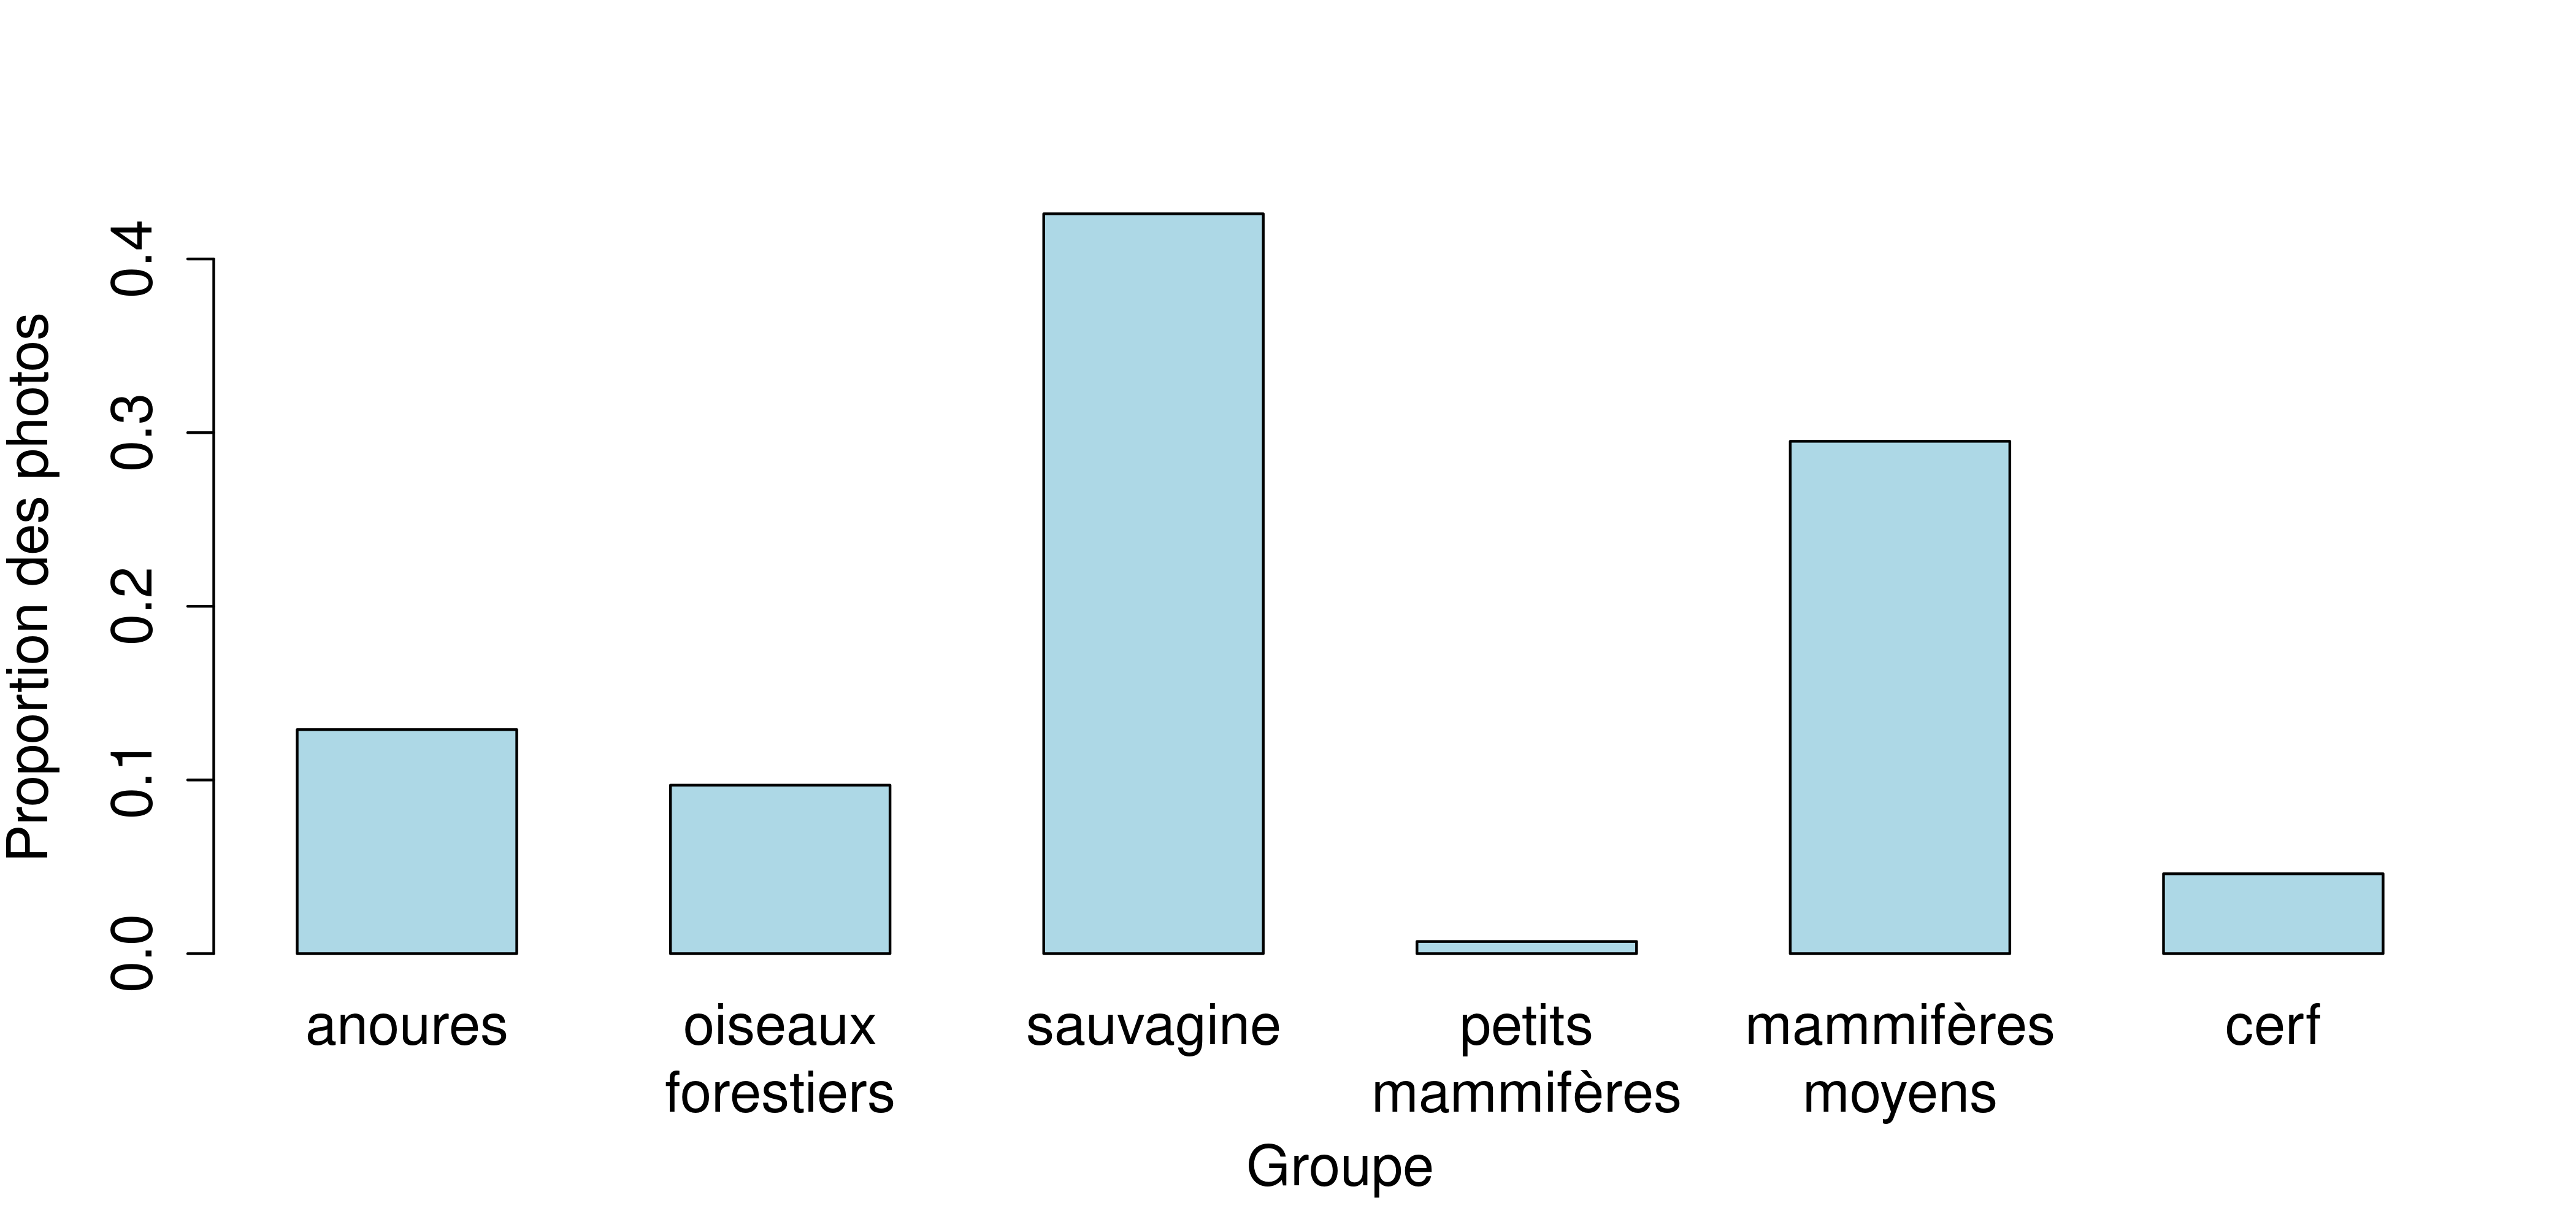
\includegraphics[width=0.9\textwidth]{fig/cam-Prop-2024.png}
\caption{Proportions des images avec détection animales de vertébrés prises par les pièges photographiques à proximité de ponceaux ou passages potentiels sur l'A10 et la route 104 en 2024. La figure a été préparée à partir des 3 400 détections animales.}
\label{fig:cam-Prop-2024}
\end{figure}


\begin{figure}
  \centering
  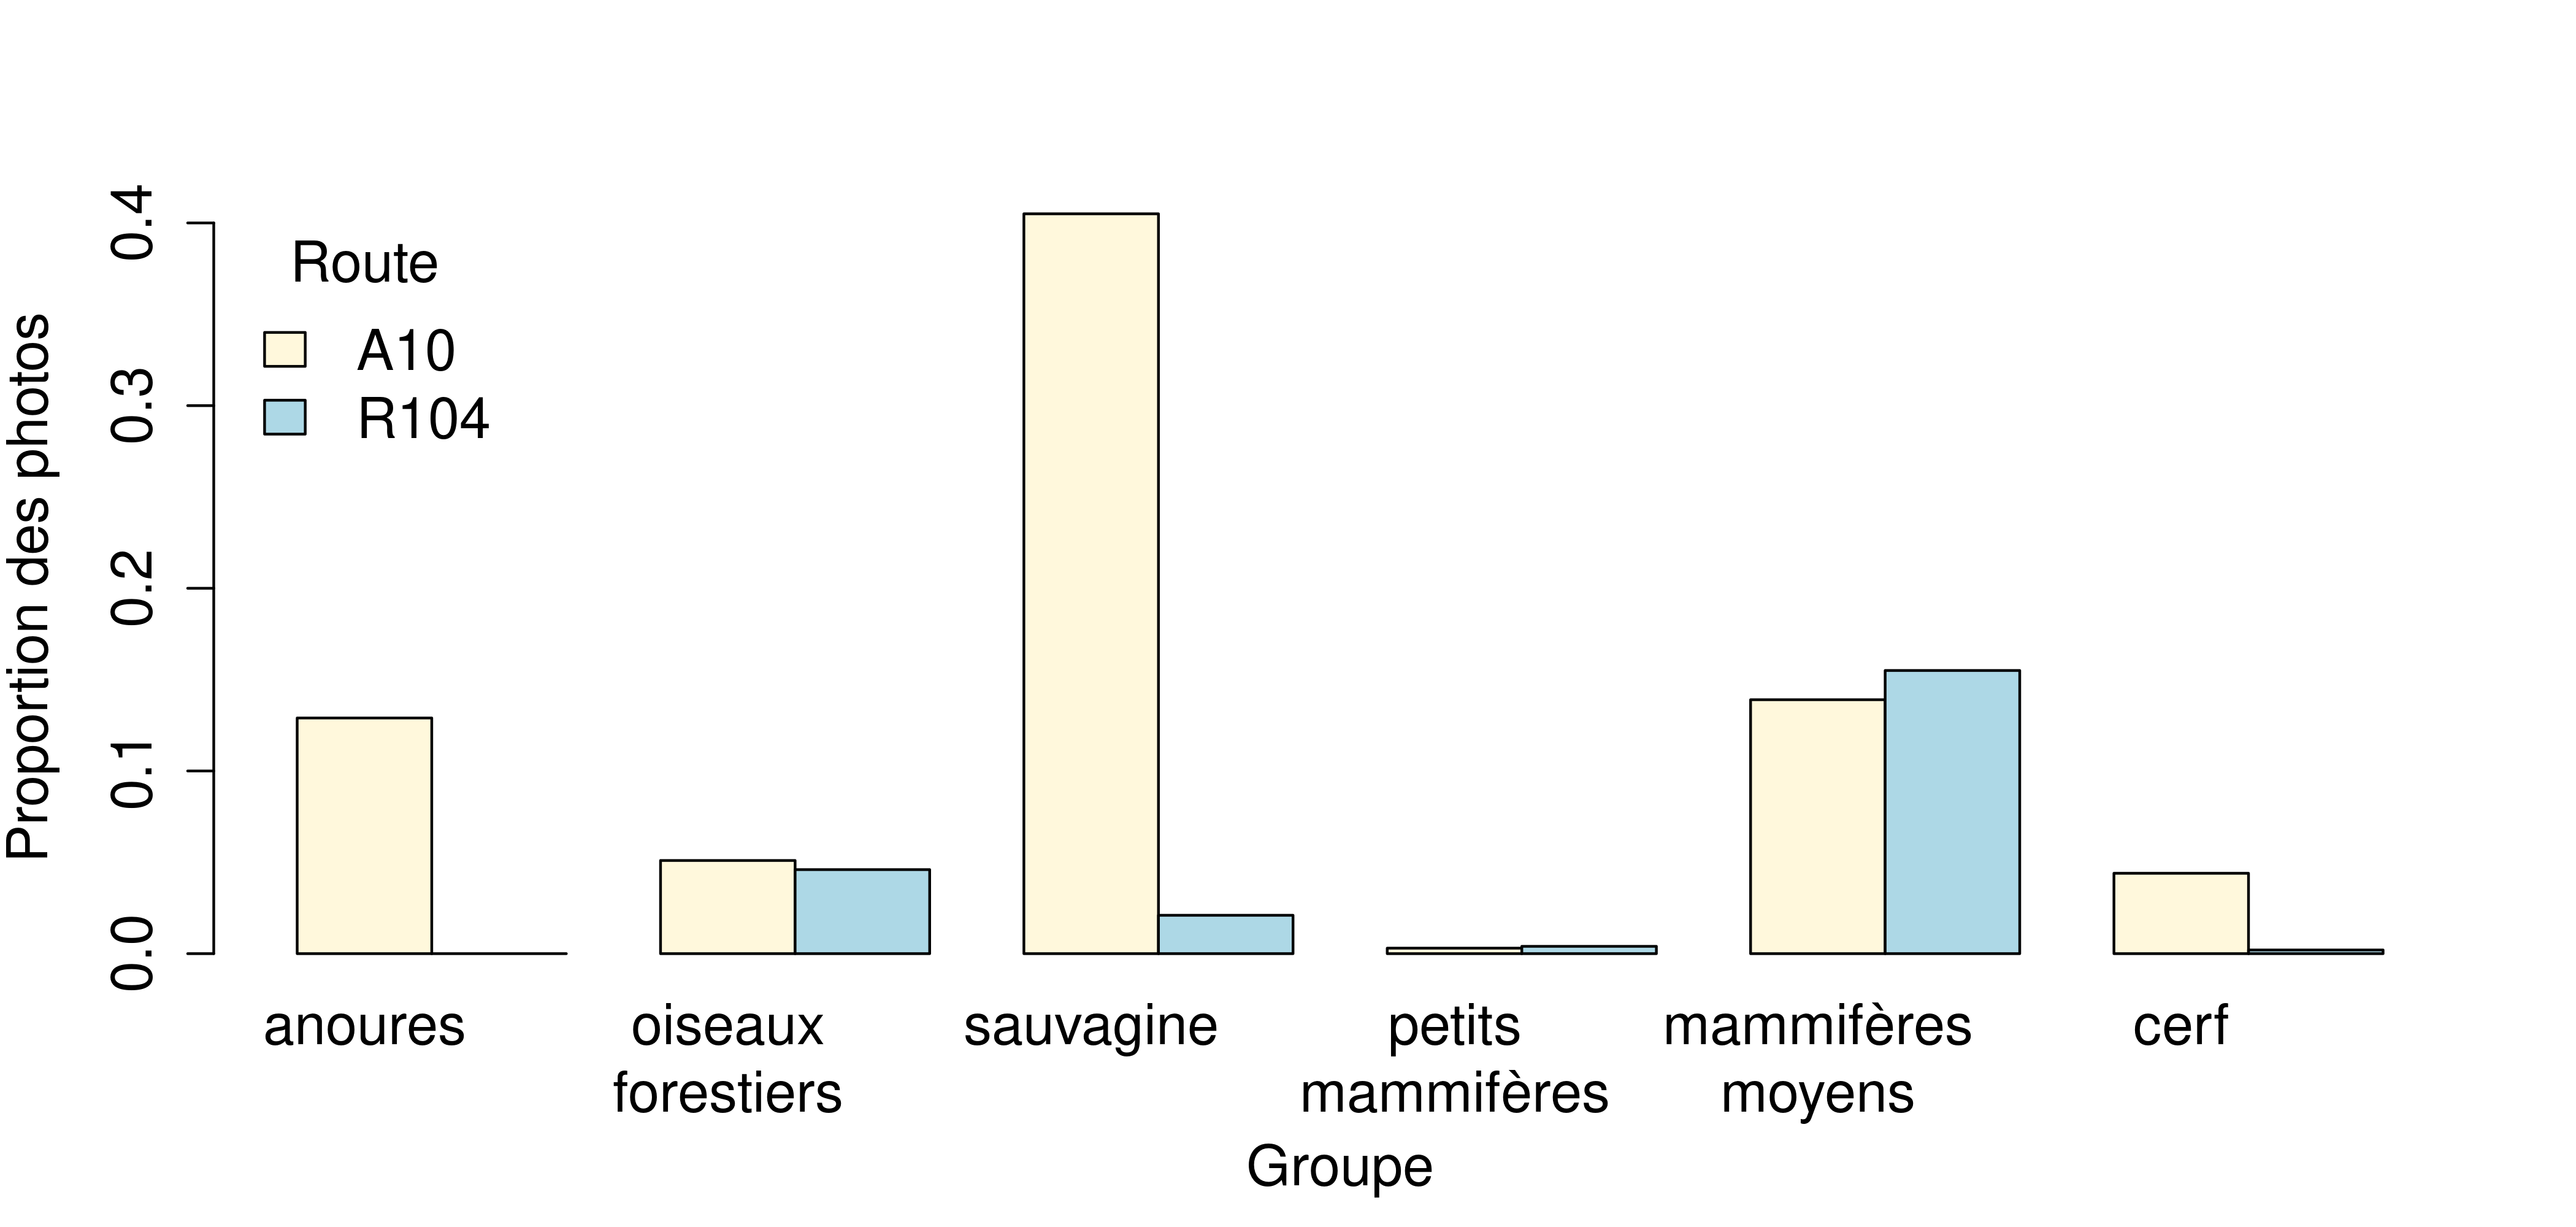
\includegraphics[width=0.9\textwidth]{fig/cam-Prop-Type-2024.png}
\caption{Proportions des images avec détection animales de vertébrés prises par les pièges photographiques dans les ponceaux à proximité de ponceaux ou passages potentiels en 2024 présentés séparément pour l'A10 et la route 104. La figure a été préparée à partir des 3 400 détections animales.}
\label{fig:cam-Prop-Type-2024}
\end{figure}


\part{Critères de connectivité écologique – Région métropolitaine de Montréal}


\section{Méthodes}

\subsection{Mortalité routière}

\subsubsection{Observation de carcasses}

En 2025, des inventaires de carcasses ont été réalisés sur 30 tronçons routiers de 1 km. Chaque tronçon faisait l'objet de deux visites, et durant chaque visite nous procédions à deux inventaires réalisés selon deux méthodes d'échantillonnage distinctes. Les inventaires se déroulaient entre 5 h 00 et 10 h 00, de manière à réduire le biais lié au retrait ou le déplacement des carcasses par les charognards et les véhicules circulant sur la chaussée.

\addM{Comme présenté au volet 1, trois méthodes ont été utilisées pour détecter les carcasses. Les inventaires par caméra embarquée ont été réalisés à l'aide de la même caméra GoPro Hero 11 Black décrite au volet 1 et avec les mêmes paramètres de configuration. La méthode à pied consistait à parcourir l’accotement en marchant. Les observateurs y repéraient, identifiaient et dénombraient toutes les carcasses détectées, y compris celles situées hors de la chaussée, sur l’accotement gravillonné ou dans la végétation herbacée en bordure de route. Sur les routes secondaires, les observateurs parcouraient successivement les deux voies en veillant à ne pas compter deux fois une même carcasse. Dans le cas où les observateurs ne pouvaient pas traverser le tronçon de manière sécuritaire, ils inventoriaient les deux voies à partir d’un seul côté de la route. Les observateurs notaient la date, l’heure, le taxon et les coordonnées géographiques de chaque carcasse à l’aide d’un GPS GARMIN GPSMAP 79s (Garmin, Schaffhausen, Suisse). La troisième méthode de détection des carcasses utilisait le même drone décrit dans le volet 1 avec les mêmes paramètres de configuration et les mêmes contraintes de conditions de vol.}
  

La méthode d'inventaire par caméra embarquée \addM{GoPro} était utilisée à chaque visite. La seconde méthode \addM{utilisée lors d'une visite donnée était soit le} \delM{de chaque visite )} \addM{drone ou le relevé à pied} \addM{et} dépendait des autorisations et des conditions de vol. Par conséquent, bien qu'une visite impliquait deux méthodes distinctes, un tronçon pouvait cumuler \addM{jusqu'à} trois méthodes différentes \delM{au bout de}\addM{après} deux visites (Tableau~\ref{tab:tab_method}).


\begin{longtable}{llrrl}
  \caption{Nombre de visites et méthodes utilisées pour les inventaires de carcasses, par tronçon.}
  \label{tab:tab_method}
  \\
  \toprule
Section & Tronçon & Catégorie & Visites & Methodes \\ 
  \midrule
T01\_E & T01 &   2 &   2 & À pied+GoPro \\ 
  T01\_O & T01 &   2 &   2 & Drone+GoPro \\ 
  T02 & T02 &   0 &   2 & À pied+GoPro \\ 
  T03\_E & T03 &   0 &   2 & À pied+Drone+GoPro \\ 
  T03\_O & T03 &   0 &   2 & GoPro \\ 
  T09\_E & T09 &   0 &   2 & GoPro \\ 
  T09\_O & T09 &   0 &   2 & À pied+GoPro \\ 
  T14\_E & T14 &   0 &   2 & À pied+GoPro \\ 
  T14\_O & T14 &   0 &   2 & À pied+GoPro \\ 
  T15\_E & T15 &   0 &   2 & GoPro \\ 
  T15\_O & T15 &   0 &   2 & À pied+GoPro \\ 
  T20\_E & T20 &   0 &   2 & Drone+GoPro \\ 
  T20\_O & T20 &   0 &   2 & Drone+GoPro \\ 
  T22\_E & T22 &   2 &   2 & À pied+GoPro \\ 
  T22\_O & T22 &   2 &   2 & GoPro \\ 
  T25\_E & T25 &   1 &   2 & À pied+Drone+GoPro \\ 
  T25\_O & T25 &   1 &   2 & GoPro \\ 
  T26\_E & T26 &   0 &   2 & GoPro \\ 
  T26\_O & T26 &   0 &   2 & À pied+GoPro \\ 
  T28 & T28 &   0 &   2 & À pied+Drone+GoPro \\ 
  T30\_N & T30 &   0 &   2 & GoPro \\ 
  T30\_S & T30 &   0 &   2 & À pied+Drone+GoPro \\ 
  T31\_E & T31 &   1 &   2 & À pied+Drone+GoPro \\ 
  T31\_O & T31 &   1 &   2 & GoPro \\ 
  T35 & T35 &   1 &   2 & À pied+Drone+GoPro \\ 
  T36 & T36 &   2 &   2 & À pied+Drone+GoPro \\ 
  T39\_E & T39 &   1 &   2 & GoPro \\ 
  T39\_O & T39 &   1 &   2 & À pied+Drone+GoPro \\ 
  T40\_E & T40 &   2 &   2 & Drone+GoPro \\ 
  T40\_O & T40 &   2 &   2 & GoPro \\ 
  T41\_E & T41 &   2 &   2 & GoPro \\ 
  T41\_O & T41 &   2 &   3 & À pied+Drone+GoPro \\ 
  T42\_E & T42 &   2 &   2 & GoPro \\ 
  T42\_O & T42 &   2 &   3 & À pied+Drone+GoPro \\ 
  T45\_N & T45 &   2 &   2 & À pied+GoPro \\ 
  T45\_S & T45 &   2 &   2 & GoPro \\ 
  T47\_E & T47 &   2 &   2 & Drone+GoPro \\ 
  T47\_O & T47 &   2 &   2 & GoPro \\ 
  T48\_E & T48 &   1 &   2 & À pied+GoPro \\ 
  T48\_O & T48 &   1 &   2 & GoPro \\ 
  T49 & T49 &   2 &   2 & À pied+Drone+GoPro \\ 
  T52\_E & T52 &   2 &   2 & GoPro \\ 
  T52\_O & T52 &   2 &   2 & À pied+GoPro \\ 
  T53\_E & T53 &   1 &   2 & GoPro \\ 
  T53\_O & T53 &   1 &   2 & À pied+Drone+GoPro \\ 
  T57\_E & T57 &   2 &   2 & Drone+GoPro \\ 
  T57\_O & T57 &   2 &   2 & GoPro \\ 
  T59 & T59 &   1 &   2 & À pied+GoPro \\ 
  T61\_N & T61 &   2 &   2 & À pied+Drone+GoPro \\ 
  T61\_S & T61 &   2 &   2 & GoPro \\ 
  T62\_E & T62 &   1 &   2 & GoPro \\ 
  T62\_O & T62 &   1 &   2 & À pied+Drone+GoPro \\ 
  T65\_N & T65 &   1 &   2 & À pied+Drone+GoPro \\ 
  T65\_S & T65 &   1 &   2 & GoPro \\ 
   \bottomrule
\label{tab:visites}
\end{longtable}


\comM{Mieux de garder ça succinct, ça ne sert à rien de s'autoplagier entre différentes sections.}\delM{(GoPro, San Mateo, Californie, États-Unis) fixée au centre de la partie avant du capot du véhicule au moyen d'un trépied magnétique 3-Footed Monster. Afin d'enregistrer la chaussée lors du parcours de chaque tronçon, la caméra était configurée en résolution 4K au format 4:3, à une cadence de 30 images par seconde. La caméra était pilotée depuis l'habitacle du véhicule au moyen de l'application Quik (GoPro, San Mateo, Californie, États-Unis) installée sur un téléphone intelligent. Les carcasses ont été dénombrées a posteriori par visionnement des enregistrements vidéo. La caméra étant équipée d'un récepteur GPS intégré, chaque carcasse détectée à l'écran a pu être géolocalisée en croisant le minutage de sa détection avec les données de position contenues dans les métadonnées des fichiers \texttt{.mp4}. Dans le cas des inventaires par caméra embarquée, les deux voies de circulation étaient systématiquement parcourues. La méthode à pied consistait à parcourir l'accotement en marchant, celui-ci étant constitué de gravel ou enherbé selon le tronçon. Les observateurs y repéraient, identifiaient et dénombraient toutes les carcasses détectées, y compris celles situées hors de la chaussée, sur l'accotement gravillonné ou dans la végétation herbacée en bordure de route. Sur les routes secondaires, les observateurs parcouraient successivement les deux voies en veillant à ne pas compter deux fois une même carcasse. Dans le cas où les observateurs ne pouvaient pas traverser le tronçon de manière sécuritaire, ils inventoriaient les deux voies à partir d'un seul côté de la route. Les observateurs notaient la date, l'heure, le taxon et les coordonnées géographiques de chaque carcasse à l'aide d'un GPS GARMIN GPSMAP 79s (Garmin, Schaffhausen, Suisse). La troisième méthode de détection des carcasses, utilisant un aéronef télépiloté (ici désigné par « drone »), venait compléter les deux méthodes précédemment présentées (suivi à pied avec jumelles et caméra fixée sur véhicule) utilisait le même drone décrit dans le volet 1 avec les mêmes paramètres de configuration et les mêmes contraintes de conditions de vol. Pour rappel, cette méthode pouvait se substituer au suivi à pied dans certaines conditions. Les journées d’échantillonnage avec drone étaient moins fréquentes que celles des deux autres méthodes, car les vols nécessitent des conditions météorologiques particulières : vents inférieurs à 30 km/h et absence de précipitations. Le drone utilisé était un DJI Mavic 3 Enterprise Thermal (DJI, Shenzhen, Chine). Celui-ci a été immatriculé par Transports Canada avant les vols, et sa plaque d'immatriculation est visible sur une des pales de l'engin. Puisque le drone pesait plus de 250 g, il était nécessaire d’obtenir une certification de base pour devenir pilote. Pendant le vol, une à trois autres personnes de l'équipe doivent être des observateurs visuels, afin de conserver un contact visuel avec l’aéronef en tout temps.}
  
\delM{Dès le lever du soleil, le drone était déployé le long de l'A10 et de la R104 une fois toutes les \addM{2--3} semaines lors des conditions optimales de vol. Les vols ont été automatisés pour que le drone effectue des tronçons linéaires, en restant parallèle aux routes et en volant à au moins 5 m de la chaussée. Les trajets de vol étaient de 500 m chacun, le but étant de voler de part et d'autre des futurs passages, soit 250 m avant et 250 m après les points définis de ceux-ci (Figure 3). L’altitude de vol était de 40 m. Nous avons utilisé deux types de caméras, une de grand-angle et une thermique. La caméra grand-angle possède une qualité d’image de 20 mégapixels, et une lentille avec un champ de vision de 84°, un équivalent format de 24 mm, une ouverture de f/2.8 et une mise au point à 1 m. La qualité du 4K permet d’obtenir 60 images par seconde. La caméra thermique de ce drone fonctionne avec un imageur thermique, le Microbolomètre VOx non refroidi et d’un spotmètre. La lentille a un champ de vision de 61°, un équivalent format de 40 mm, une ouverture de f/1.0 et une mise au point à 5 m. La plage de mesure va de -20° à 150°C, avec une précision de +/- 2°C.
Le drone circulait à une vitesse de 2 m/s, afin de bien couvrir la chaussée lors du visionnement. La caméra du drone était orientée à 90 degrés pour faire face à la route et agrandissait l’image continuellement à un grossissement de X2. Les fichiers vidéo des vols de 500 m de qualité 4K (ratio d’image en 4:3) ont été visionnés en laboratoire et les données d'observation sur la route ont été saisies en notant le moment (minutes, secondes) de la séquence vidéo. Les carcasses ont été géolocalisées, au même titre que les deux précédentes méthodes. 
Le but de cette technique était de mettre en relation les données d'inventaire sur la faune retrouvée proche des futurs passages fauniques et les individus retrouvés morts sur la route. }



\subsubsection{Persistance de carcasses sur la route}

Afin d'estimer la durée de présence d'une carcasse avant son enlèvement par les charognards, nous avons réalisé des tests de persistance sur la majorité des tronçons suivis \addM{en suivant le même protocole que décrit dans le volet 1}. \delM{Ainsi, à}\addM{À partir} du mois de juin, deux tests hebdomadaires étaient effectués, chacun sur un tronçon différent. L'un débutait après le lever du soleil (vers 5h00), l'autre un peu avant le coucher du soleil (vers 20h00). L'emplacement (la voie et le kilométrage) de chaque test était tiré aléatoirement. Lors de chaque test, des morceaux de poulet cru de 1.5 cm x 3 cm x 3 cm étaient déposés sur l'accotement et suivis par un piège photographique paramétré pour capturer une image toutes les 15 secondes. La caméra, une Spypoint Force-20, était montée sur un pivot à une hauteur standard de 30 cm du sol, fixé à un piquet de bois lui-même stabilisé par des planches à sa base. Après environ 24 heures suivant son déploiement, la caméra était retirée. L'heure et la date de pose de la caméra, l'heure et la date de retrait, les coordonnées, et le cas échéant le temps écoulé entre la pose et la prédation ainsi que l'identité du charognard, étaient consignés.



\subsubsection{Observations complémentaires}
\comM[inline]{Est-ce pertinent de maintenir une sous-sous-section \og Observations complémentaires \fg{}? Il n'y a rien dans la section pour le moment.}

\subsection{Suivi de la petite faune}

\subsubsection{Pièges photographiques}

Des pièges photographiques (GardePro T5CF, Hong Kong, Chine) ont été installés en mai 2025 à chacun des 30 tronçons sélectionnés. Un appareil a été disposé à proximité d'un ponceau dans chaque tronçon. \addM{Nous avons utilisé les mêmes paramètres de configuration que décrits dans le volet 1.} Ces pièges photographiques ont permis de détecter la faune, et plus particulièrement les mammifères de petite et moyenne taille, ainsi que l'herpétofaune. Ces pièges photographiques ont été retirés en octobre 2025. \delM{Les pièges photographiques ont été programmés avec deux modes de déclenchement: la prise de photo à intervalle régulier de 5 minutes (\emph{time lapse}) pour les ectothermes et la prise d'une photo après détection de mouvement pour les endothermes. Afin de ne pas saturer le stockage des cartes mémoires, nous avons réglé la qualité à 4 mégapixels. Le principal avantage du modèle de caméra que nous avons choisi est la mise au point rapprochée des animaux détectés avec un focus à 20 cm, facilitant l'identification des petits organismes.}

\addM{Nous avons utilisé l'outil MegaDetector pour traiter les images récoltées, en suivant la même approche que pour le volet 1.} \delM{Cet outil permet de trier les images qui contiennent des photos avec animaux et de celles qui n'en contiennent pas. MegaDetector n'identifie pas à l'espèce. C'est pour cette raison que les} \addM{Les images avec détection présumée et avec une confiance $\geq 75$\% ont ensuite été validées par un humain pour déterminer si la détection était avérée et le cas échéant, d'identifier les individus dans les images au taxon le plus bas possible.}
  
\delM{Dans un premier temps, nous avons utilisé l'outil de reconnaissance automatique MegaDetector afin de faire un tri initial des photos en deux catégories: avec animal et sans animal} \delM{Cet outil disponible gratuitement repose sur l'architecture YOLO version 5 basée sur des réseaux de neurones convolutionnels et a été entraîné par Microsoft à reconnaître différents taxons. MegaDetector n'identifie pas les éléments de l'image à l'espèce, mais catégorise plutôt les éléments comme étant des animaux ou non. Pour chaque élément identifié dans une image, MegaDetector lui attribue une probabilité à être dans la bonne catégorie (i.e., animal ou non). Nous avons lancé MegaDetector sur un serveur de calcul dédié du laboratoire du professeur Mazerolle à l'Université Laval.}

\delM{Afin de réduire le nombre de faux positifs, nous avons filtré les images pour lesquelles la probabilité était $\geq 75$\%. Nous avons visionné chacune de ces images afin de valider si la détection était avérée et le cas échéant, nous avons identifié les individus sur les images au taxon le plus bas possible (famille, genre ou espèce). Ces informations ont ensuite été utilisées pour évaluer l'occurrence de différents taxons à proximité des ponceaux. De plus, ces images annotées serviront à l’entraînement d’algorithmes d’intelligence artificielle pour la reconnaissance à l'espèce, notamment à l’aide du logiciel YOLO version 11.}


\subsubsection{Enregistrements acoustiques}

Nous avons installé 18 enregistreurs acoustiques automatisés à la fin avril 2025 aux milieux humides près des tronçons, présentant des habitats favorables à l’occupation \addM{par} des anoures (AudioMoths; \citealt{hill2019}). Ces appareils étaient placés à environ 1,5 m du sol et fixés à des arbres ou à des poteaux. Les appareils ont été programmés pour enregistrer les sons durant trois minutes, à cinq reprises dans la journée (20h00, 00h00, 7h00, 10h00, 14h00). Ces plages sont celles pendant lesquelles différentes espèces d’anoures sont actives, incluant la rainette faux-grillon (\emph{Pseudacris triseriata}) \citep{fayard2022}. Ces enregistreurs ont été retirés à la fin octobre 2025, à l'exception des enregistreurs sur T20, T48, T49\_1 et T57 qui ont été retirés à la fin juillet ou en août 2025 (Tableau \ref{tab:tab_AM25}).

Les plages d'enregistrement ont été analysées à l’aide de BirdNET, un outil de reconnaissance automatique utilisant l’intelligence artificielle \citep{kahl2021}. Cet outil permet d’identifier sur chaque enregistrement sonore les espèces pour lesquelles il a été entraîné. Les enregistreurs acoustiques nous ont permis de suivre les périodes de reproduction des anoures aux sites où l’accès est plus difficile pour le suivi visuel (longue distance à faire à pied, stationnement interdit en bordure d’autoroute), mais également de déterminer les espèces qui se reproduisent à proximité des tronçons à l'étude.

Bien que le modèle BirdNET soit déjà entraîné à reconnaître dix des espèces d'anoures présentes au Québec, deux espèces ne sont pas prises en charge par l’algorithme : la grenouille du Nord (\emph{Lithobates septentrionalis}) et la grenouille léopard (\emph{Lithobates pipiens}). Afin d’assurer une détection exhaustive des anoures, nous avons donc utilisé une version personnalisée de BirdNET que nous avons entraînée dans le laboratoire du professeur Mazerolle pour ces deux taxons. Cet entraînement reposait sur un corpus de 2 142 extraits acoustiques d’une durée de trois secondes chacun, préalablement sélectionnés et validés à la main. Les données provenaient de plateformes de science participative, notamment Xeno-canto, iNaturalist et Macaulay Library et extraites à l’aide du package R suwo \citep{arya-salas2025suwo}. Nous avons complété ce corpus d'entraînement avec des enregistrements issus de travaux antérieurs du laboratoire de biologie de la conservation quantitative du professeur Mazerolle. Une attention particulière a été portée à l’équilibrage du jeu d’entraînement afin de limiter les biais et le surapprentissage associés à certaines catégories de sons. Les 2 142 extraits étaient répartis en neuf classes distinctes (Tableau~\ref{tab:tab_clips}).


\begin{table}[H]
\centering
\caption{Composition du corpus d'entraînement du modèle de classification personnalisé BirdNET. Chaque clip a une durée de 3 secondes. Les clips ont été extraits à partir de fichiers audios issus des bases de données de sciences participatives (Xeno-canto, iNaturalist et Macaulay) et de la collection sonore du laboratoire du professeur Mazerolle.}
\label{tab:tab_clips}
\begin{tabular}{lrl}
  \hline
Classe & Nombre de clips (3s) & Description  \\ 
  \hline
ANTHRO & 124 & Bruits d'origine anthopique (moteurs et véhicules) \\
BIRDS & 247 &  Vocalisation d'oiseaux \\
CLAMITANS & 250 &  \emph{Lithobates clamitans} (Grenouille verte) \\
CRUCIFER & 250 &  \emph{Pseudacris crucifer} (Rainette crucifère) \\
PIPIENS & 242 &  \emph{Lithobates pipiens} (Grenouille léopard) \\
SEPTENTRIONALIS & 284 & \emph{Lithobates septentrionalis} (Grenouille du Nord) \\
SILENCE & 245 &  Clips sans signal biologique \\
VERSICOLOR & 250 & \emph{Dryophytes versicolor} (Rainette versicolore) \\
WEATHER & 250 &  Bruits météorologiques (vent et pluie) \\
     \hline
\end{tabular}
\end{table}

Nous avons évalué les performances du modèle personnalisé à partir d'un ensemble indépendant de 386 clips audio de 3 secondes, représentant environ 20 \% du corpus d'entraînement. \delM{Notons que cette proportion ne correspond à aucun seuil documenté.} \delM{Elle résulte simplement}\addM{Ceci correspondait à} un compromis entre \addM{le} nombre d'extraits suffisant pour obtenir des résultats concluants et \addM{la disponibilité} des données accoustiques. Cet ensemble comprenait des clips de grenouille du Nord et de grenouille léopard, ainsi que des clips négatifs (bruits environnementaux sans grenouille du Nord ou grenouille léopard) afin de tester la capacité du modèle à discriminer les deux espèces cibles du bruit de fond. Afin de garantir l’indépendance de l’évaluation, nous avons veillé à ce que ces clips soient issus de fichiers qui n’avaient pas servi à entraîner BirdNET en amont. \delM{Toutefois,}\addM{La validation sur un jeu de données délimité est un premier pas, mais ne reflète} pas pleinement le comportement réel du modèle en situation réelle. \addM{En effet, une meilleure évaluation devrait utiliser un plus grand volume de données}\delM{où ce dernier est exposé à un volume de données considérablement plus important}, à une plus grande variabilité acoustique et à des sons pour lesquels il n'a pas été entraîné.\delM{, augmentant ainsi le risque de faux positifs.} Il est donc attendu que notre modèle personnalisé produise encore un nombre élevé d'erreurs à ce stade. Ce taux devrait diminuer au fur et à mesure de l'entraînement, l'objectif étant d'obtenir un outil suffisamment fiable pour réduire considérablement le temps consacré à l'identification des espèces dans les fichiers acoustiques.

Malgré la présence de faux positifs\addM{, le modèle a démontré des performances satisfaisantes pour les deux espèces cibles, avec une exactitude (proportion de prédictions vraies sur l’ensemble des prédictions) supérieure à 0,70 pour les deux seuils testés, particulièrement pour la grenouille Nord} (Tableau~\ref{tab:tab_confusion_pipiens}; Tableau~\ref{tab:tab_metrics_pipiens_025}; Tableau~\ref{tab:tab_confusion_pipiens_075}; Tableau~\ref{tab:tab_metrics_pipiens_075}; Tableau~\ref{tab:tab_confusion_septentrionalis_025}; Tableau~\ref{tab:tab_metrics_septentrionalis_025}; Tableau~\ref{tab:tab_confusion_septentrionalis_075}; Tableau~\ref{tab:tab_metrics_septentrionalis_075}). Ces résultats indiquent que le modèle peut être utilisé comme outil de présélection des détections, réduisant substantiellement le temps de validation par rapport à l'écoute intégrale des enregistrements\addM{, à condition que les détections retenues fassent l'objet d'une validation manuelle}. Les faux positifs observés s'expliquent en partie par la similarité entre les vocalisations de \emph{L. septentrionalis} et celles d'autres espèces, notamment \emph{L. sylvaticus}. La constitution d'un corpus d'entraînement plus étoffé, incluant des enregistrements printaniers et estivaux de 2026, permettront d’améliorer les performances du modèle.

Avant l’analyse des fichiers audios, nous avons exclu les enregistrements affectés par des conditions météorologiques défavorables (vents forts et précipitations intenses) afin de préserver la qualité des données. Pour ce faire, nous avons utilisé notre modèle personnalisé préalablement entraîné pour la grenouille du Nord et la grenouille léopard, capable de détecter la présence de vent et de pluie à partir du signal acoustique (Tableau \ref{tab:tab_clips}). Nous avons utilisé ce modèle sur l'ensemble des enregistrements pour filtrer les enregistrements de mauvaise qualité. Ainsi, tout fichier contenant au moins un clip de 3 secondes classé dans la catégorie de mauvaise qualité (i.e., WEATHER, voir Tableau \ref{tab:tab_clips}) avec un score de confiance supérieur ou égal à 0,75 a été retiré des analyses subséquentes.

\subsubsection{Recherche par drone}

Comme en 2024, nous avons réalisé des suivis par drones au-dessus des zones humides de l'A10 et de la R104, afin de détecter les tortues qui thermorégulent dans les milieux humides \citep{aota2021, bogolin2021, bevan2018}. Nous avons utilisé le même drone décrit plus haut pour ces inventaires, en suivant le même protocole pour les observateurs visuels. \delM{Cette technologie permet d'éviter l'effarouchement des tortues, en respectant les recommandations de vol à une altitude minimale de 20 m au-dessus des milieux humides. Les survols en drone permettent aussi une couverture complète de la zone d’inventaire, et facilitent l’accès à des secteurs qui auraient été inaccessibles à pied.}

\delM{Transports Canada réglemente les zones où le vol de drone est autorisé. La zone de vol doit se situer à plus de 9 km de tout aéroport, héliport ou aérodrome. De même, les vols sont interdits au-dessus d’espaces réglementés, comme une base militaire, une prison ou une aire protégée comme celle du Bois de Brossard.} Les secteurs d’inventaire que nous avons sélectionnés \addM{n’étaient pas soumis à des interdictions de vols associées à la proximité d'espaces réglementés par Transports Canada}\delM{avaient pas de contrainte de vol}. \delM{Nous avons cherché des aires de décollage et d’atterrissage sécuritaires.} Ces suivis ont été réalisés à différentes périodes de la saison d'activité des tortues entre mai et octobre \delM{2024}\comM[inline]{C'était bien en 2025, non?}\addM{2025} \citep{boyer1965, obbard1981, lefevre1995}.

\delM{Nous avons suivi la méthodologie de recherche active proposée dans le protocole standardisé de détection et d'identification des tortues d'eau douce à l'aide de drones au Québec}\addM{Comme décrit dans le volet 1, nous avons suivi le protocole de recherche active proposé pour la détection et l'identification des tortues d'eau douce au Québec} \citep{mffp2021}. \delM{Nous avons rempli le "formulaire de prise de données" figurant dans l'annexe C de ce même protocole après chaque sortie. Les sorties se faisaient selon les conditions météorologiques suivantes : journée ensoleillée et couverture nuageuse pouvant aller jusqu’à 75 \%, température de l’air entre 10 et 25 \textdegree C, journée sans vent ou jusqu’à une légère brise (niveau 2 sur l’échelle de Beaufort). La caméra thermique du drone était utilisée pour connaître la température des tortues observées, leur substrat ainsi que l’eau du milieu où elles se trouvaient. Pendant une mission de vol, les milieux humides ont été survolés à basse vitesse à une altitude variant de 30 à 40 m. Lorsqu'une forme ressemblant à une tortue était repérée, nous avons utilisé le zoom du drone allant jusqu'à un grossissement de 56x pour confirmer qu'il s’agissait d'une tortue. En plus de la recherche active, lors d’une même visite nous avons lancé des vols automatisés qui filmaient l’intégralité du milieu humide en suivant toujours le même chemin à une altitude fixe de 40 m et un angle de caméra fixé à 90 \textdegree. Le but des vols automatisés était de constituer une banque de vidéos qui pourront servir à entraîner une intelligence artificielle (IA) pour identifier les tortues de manière automatique. Étant donné que la recherche active est plus longue que les vols automatisés,  nous voudrions utiliser l’IA sur les vols automatisés de tous les sites suivis.}



\subsubsection{Stations de plaques à reptiles}

Selon le même dispositif que celui décrit dans la méthode de la partie I, 22 stations de plaques à reptiles ont été installées et réparties parmi\delM{entre} les 30 tronçons entre le 5 et le 30 mai 2025. \delM{Nous n'avons pas pu attribuer une station de plaques à reptiles par tronçon, car parfois}\addM{Il a été impossible d'installer des plaques à reptiles dans certains tronçons où le milieu était défavorable aux couleuvres.} Sur les 22 \delM{stations installées}\addM{tronçons avec une station}\comM{Pas clair si 1 station = 1 tronçon. Il faut le dire clairement.}, trois visites ont été effectuées en 2025 : une au printemps, une durant l'été et une à la fin de l'été\comM[inline]{Ça prendrait des plages de dates pour quantifier \og printemps \fg{}, \og été \fg{} et \og fin d'été \fg{}.}. Les installations \delM{étaient}\addM{ont été} démantelées durant l'automne 2025.


\section{Résultats}

\subsection{Mortalité routière}

\subsubsection{Observation de carcasses}





\subsubsection{Persistance de carcasses sur la route}


\subsubsection{Observations complémentaires}



\subsection{Suivi de la petite faune}

\subsubsection{Pièges photographiques}
Un total de \mbox{2 584 774} images prises en 2025 sur les trente ponceaux à l'étude ont été traitées par MegaDetector, nécessitant \mbox{5 780 601} secondes de temps de calcul, équivalant à 66.9 jours de calcul en continu. À partir de ces images traitées, nous avons terminé la validation des images de 18 ponceaux, ce qui représente 54\% des photos du jeu de données. Nous avons inspecté les 38 110 images étiquetées par MegaDetector comme ayant des détections animales pour lesquelles la confiance était $\geq 75$\% dans ces 18 ponceaux. La validation de ces images par un humain a révélé que le taux de vrais positifs était de 45.95\%: 19 090 des détections étaient de vraies détection d'animaux. Le taux de faux positifs était de 54.05\% (i.e., détections présumées par MegaDetector mais non avérées). À partir des 38 110 images étiquetées par MegaDetector, nous avons également noté des faux-négatifs, c'est-à-dire, des sections d'images où MegaDetector n'avait pas déclaré la présence d'un animal. À partir de l'inspection des images des 18 ponceaux pour lesquelles le seuil de confiance $\geq 75$\%, nous avons détecté 2 465 animaux additionnels. Un total de 39 121 détections animales ont été répertoriées sur les 1 395 515 images des 18 ponceaux.

Différents groupes et espèces ont été observées sur les images, incluant des invertebrés (araignées, odonates, papillons) et plusieurs vertébrés (Tableau \ref{tab:cam-sp}). Des 39 121 détections animales, 78\% étaient des mammifères de moyenne taille et 13\% étaient de la sauvagine. Les autres animaux détectés étaient des oiseaux forestiers (7\%), des petits mammifères (1\%), des reptiles (0.2\%) et des amphibiens (0.6\%) (Fig. \ref{fig:cam-Prop}. La répartition actuelles des observations selon les types de tronçons ne suggère pas de patrons particuliers pour le moment, mis à part les petits mammifères qui semblaient plus fréquents dans les tronçons de catégorie 2 (milieu humide de chaque côté), bien qu'il reste environ 50\% des images à valider (Fig. \ref{fig:cam-Prop-Type}).

\begin{table}
  \caption{Espèces et groupes d'espèces répertoriées sur les images prises par les pièges photographiques dans les ponceaux des tronçons suivis en 2025. Le tableau a été préparé à partir des 39 121 détections animales provenant des 18 tronçons analysés.}
  \label{tab:cam-sp}
  \begin{tabular}{p{0.3\textwidth}p{0.7\textwidth}}
    \hline
    Groupe & Espèces ou niveau taxonomique supérieur \\
    \hline
    Amphibiens & Anoures (\emph{Lithobates} sp.) \\
    Reptiles & Couleuvres et tortues (\emph{Chelydra serpentina}) \\
    Oiseaux forestiers & Passereaux et dindon sauvage (\emph{Meleagris gallopavo}) \\
    Sauvagine & Canards, bernaches (\emph{Branta canadensis}) et échassiers (grand héron \emph{Ardea herodias}, héron vert \emph{Butorides virescens}, bihoreau gris \emph{Nycticorax nycticorax}) \\
    Petits mammifères & Écureuil roux (\emph{Tamiasciurus hudsonicus}), écureuil gris (\emph{Sciurus carolinensis}), musaraigne (\emph{Sorex} sp.), polatouche (\emph{Glaucomys} sp.), souris (\emph{Zapus hudsonius} ou \emph{Napaeozapus insignis}), campagnols (\emph{Microtus pennsylvanicus} ou \emph{Clethrionomys gapperi}), tamia rayé (\emph{Tamias striatus}) \\
    Mammmifères moyens & castor du Canada (\emph{Castor canadensis}), chat domestique (\emph{Felis catus}), chien domestique (\emph{Canis familiaris}), lièvre d’Amérique (\emph{Lepus americanus}), loutre de rivière (\emph{Lontra canadensis}), marmotte commune (\emph{Marmota monax}),  mouffette rayée (\emph{Mephitis mephitis}), \emph{Mustela} sp., opossum de Virginie (\emph{Didelphis virginiana}), rat surmulot (\emph{Rattus norvegicus}), raton laveur (\emph{Procyon lotor}, rat musqué (\emph{Ondatra zibethicus}), renard roux (\emph{Vulpes vulpes}), vison d'Amérique (\emph{Vison vison}) \\
    Grands mammifères & Cerf de Virginie (\emph{Odocoileus virginianus}) \\
    Invertébrés & Araignées, lépidoptères et odonates \\
   \hline
  \end{tabular}
\end{table}


\begin{figure}
  \centering
  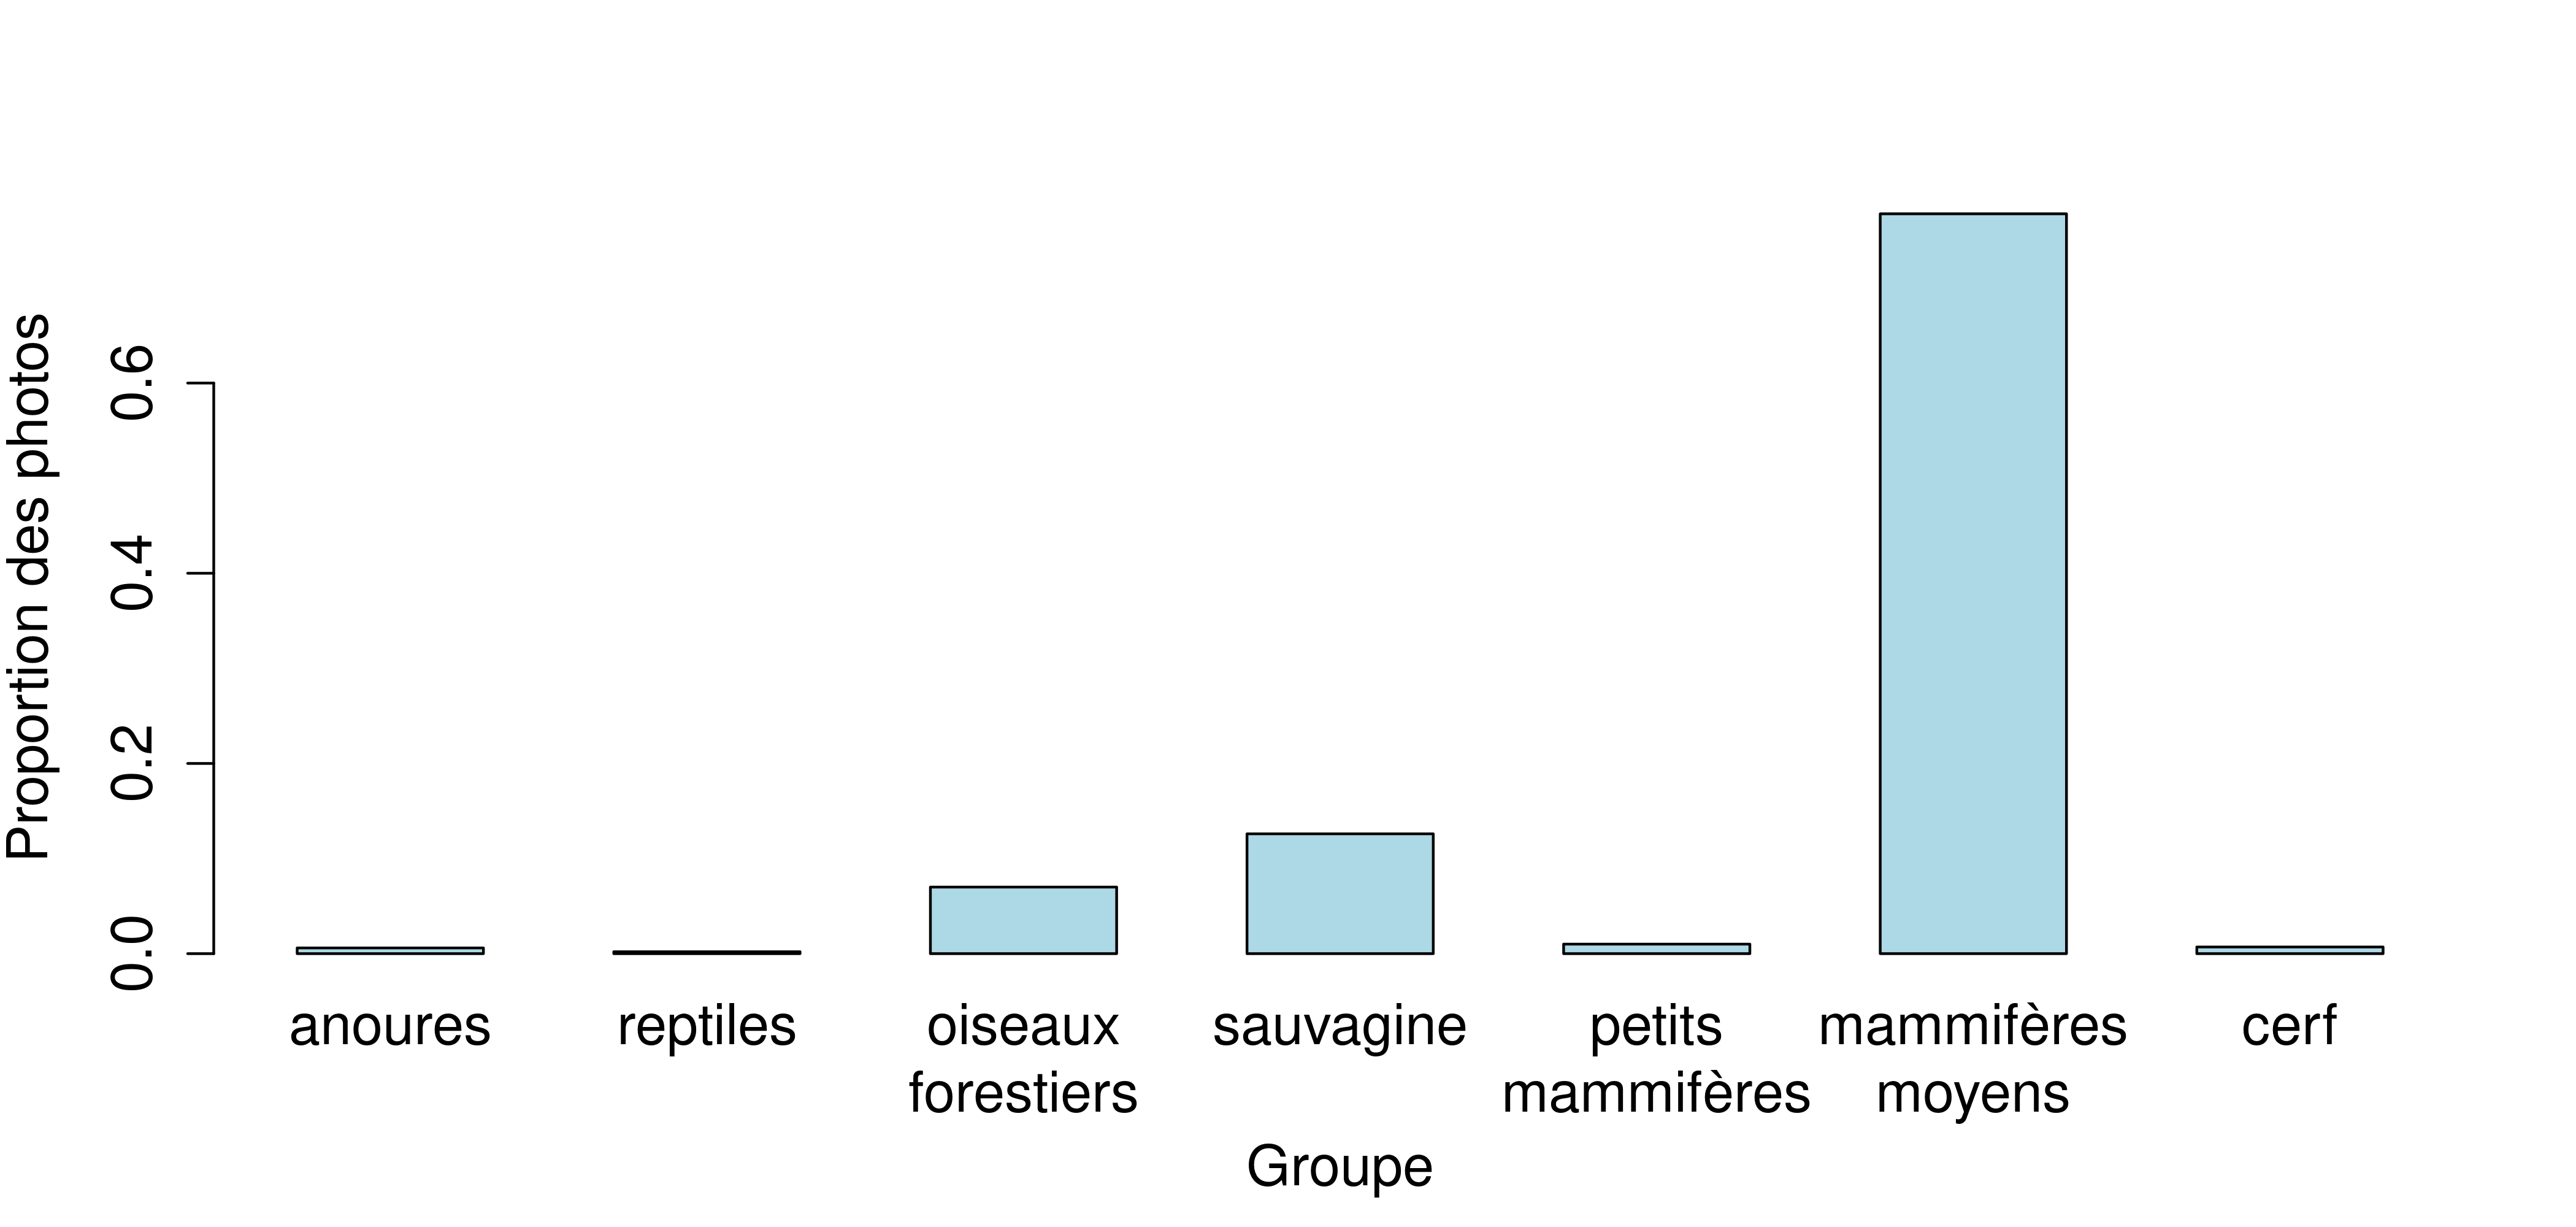
\includegraphics[width=0.9\textwidth]{fig/cam-Prop.png}
\caption{Proportions des images avec détection animales de vertébrés prises par les pièges photographiques dans les ponceaux des tronçons suivis en 2025. La figure a été préparée à partir des 39 121 détections animales provenant des 18 tronçons analysés.}
\label{fig:cam-Prop}
\end{figure}


\begin{figure}
  \centering
  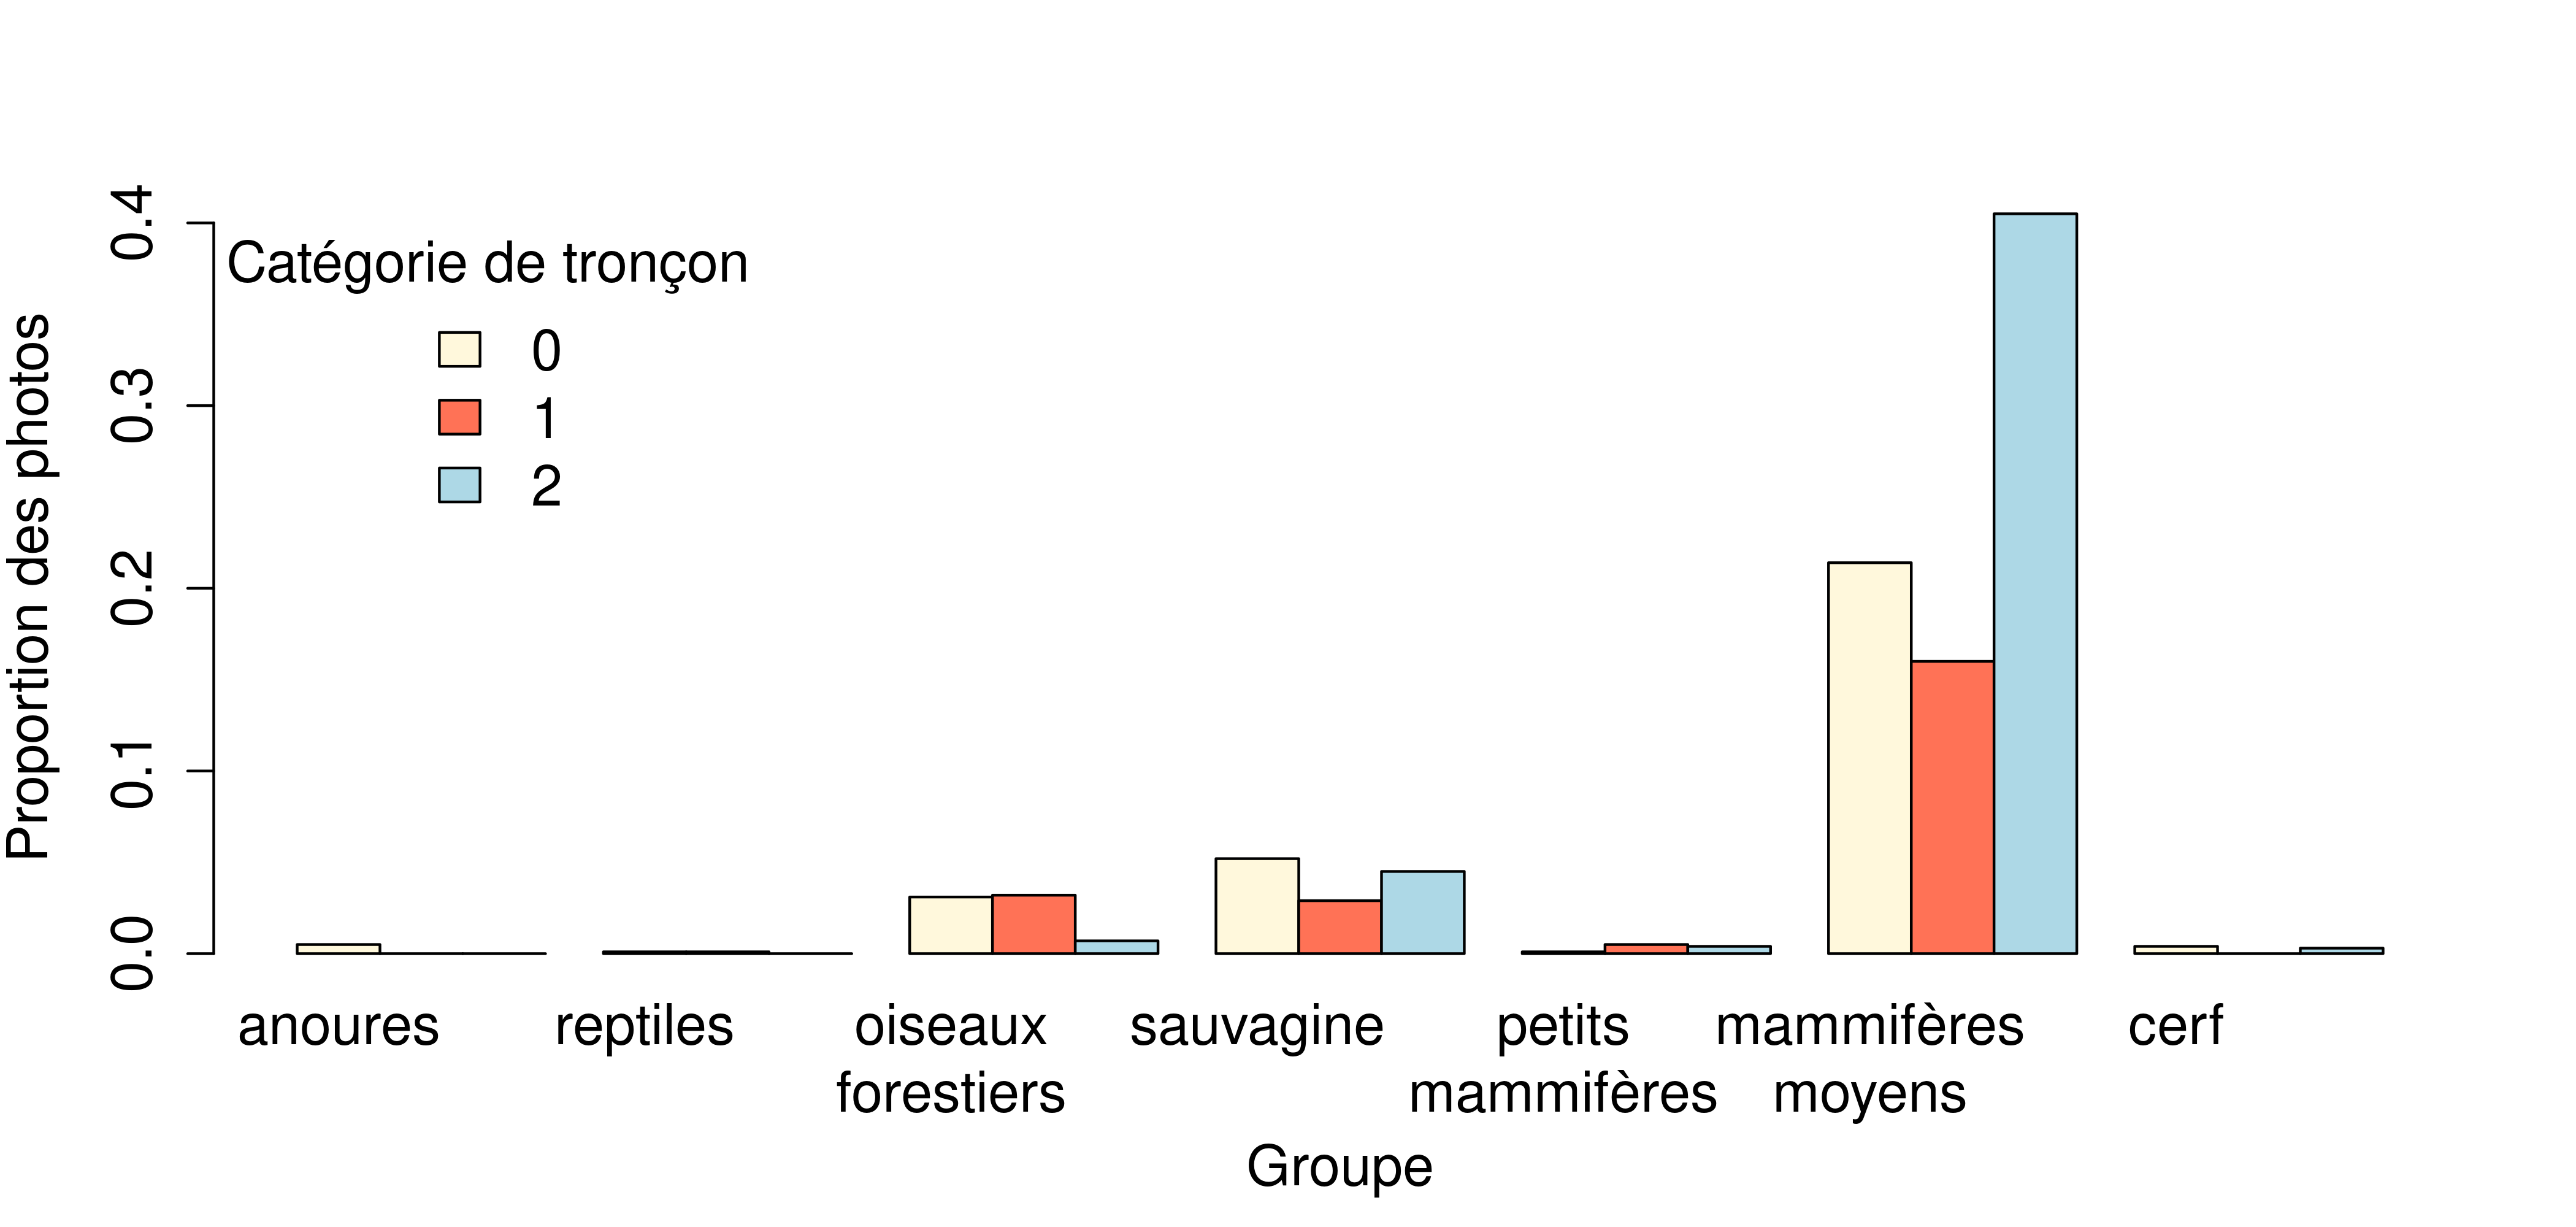
\includegraphics[width=0.9\textwidth]{fig/cam-Prop-Type.png}
\caption{Proportions des images avec détection animales de vertébrés prises par les pièges photographiques dans les ponceaux des tronçons suivis en 2025 selon les trois différentes types de tronçons échantillonnés. La figure a été préparée à partir des 39 121 détections animales provenant des 18 tronçons analysés.}
\label{fig:cam-Prop-Type}
\end{figure}






\subsubsection{Enregistrements acoustiques}



\subsubsection{Recherche par drones}





\subsubsection{Stations de plaques à reptiles}

\section{Discussion}

\subsection{Mortalité routière}

\subsubsection{Observation de carcasses}

Ces premiers résultats mettent en évidence la faible efficacité du drone et de la GoPro, comparativement à la méthode à pied, pour détecter les carcasses sur la chaussée (Fig.~\ref{fig:bar_mix_25}). La méthode par drone avait d'ailleurs été retirée du protocole pour l'échantillonnage de 2026, faute de détection en 2025. Les résultats issus des GoPro sont toutefois à nuancer. En effet, bien que peu performante par rapport à la méthode à pied, cette méthode a tout de même permis de détecter des carcasses de mammifères. Sur les six carcasses observées, une était une marmotte, deux des moufettes, deux des ratons laveurs et une dernière un mammifère indéterminé. En revanche, les enregistrements n'ont permis de détecter aucun anoure, oiseau ou reptile. Ainsi, dans le cadre de cette étude, seule la méthode à pied a permis de détecter l'ensemble des groupes de vertébrés, la GoPro se limitant aux vertébrés de taille moyenne.

Le protocole initial prévoyait d'associer aux inventaires par enregistrement GoPro des inventaires réalisés par observation directe depuis le véhicule. Cette combinaison devait permettre de quantifier la perte d'information entre le visionnement différé des enregistrements et le dénombrement des carcasses en temps réel. Les auxiliaires de recherche n'ont toutefois pas été en mesure d'appliquer conjointement les deux protocoles, de sorte que cette information ne pourra être obtenue dans le cadre des tronçons suivis actuellement. 

Des données quantitatives sur cette perte d'information devraient néanmoins être disponibles prochainement, puisque dans le cadre d'une collaboration avec un projet de suivi de la mortalité routière amorcé au printemps 2026 sur un tronçon de 14 km de l'autoroute 35, entre Saint-Sébastien et Saint-Armand. Ce projet vise notamment à quantifier la mortalité routière de l'herpétofaune dans ce secteur. Depuis le 19 mai 2026, deux auxiliaires de recherche y inventorient et dénombrent les carcasses présentes sur la chaussée selon trois méthodes. La première consiste à parcourir à pied les abords de la chaussée sur une section de 4,5 km, et ce, dans chaque sens de circulation. La deuxième couvre l'ensemble du tronçon de 14 km en véhicule. La troisième repose sur l'analyse différée des enregistrements d'une caméra GoPro fixée au véhicule durant l'inventaire en véhicule, ce qui permet de comparer directement les deux dernières méthodes. Au total, 206 visites ont été réalisées.

Bien que le visionnement des enregistrements GoPro reste à faire, il est déjà possible d'établir un premier comparatif entre les observations obtenues à pied et celles obtenues lors des parcours en véhicule sur le tronçon de l'A35 (Fig.~\ref{fig:bar_hor_bino26}). Ce portrait fait ressortir un profil semblable à celui observé lors de la phase II du projet R875. Les inventaires en véhicule ont ainsi permis de détecter très peu d'amphibiens, de reptiles et d'oiseaux, mais ont mené au dénombrement de 267 carcasses de mammifères. Comme dans le cas du projet R875, la majorité des mammifères détectés appartenaient à des espèces de taille moyenne, notamment le raton laveur (\textit{Procyon lotor}), l'opossum d'Amérique (\textit{Didelphis virginiana}) et la moufette rayée (\textit{Mephitis mephitis}).

Il importe toutefois de souligner que les inventaires en véhicule sur l'A35 ont été réalisés sur une distance de 14 km, soit une longueur nettement supérieure à celle des tronçons de 1 km utilisés dans le projet R875.1. Le tronçon de l'A35 était également visité à 52 reprises, un effort incomparable à celui effectué sur les tronçons du R875.1. Il est donc normal d'avoir des effectifs nettement supérieurs sur l'A35. De plus, les inventaires à pied sur l'A35 ont été effectués sur une section plus courte, afin d'être réalisables pour une petite équipe. Même si les conditions ne sont pas optimales pour comparer formellement les deux méthodes. Bien que ces conditions ne permettent pas une comparaison formelle des deux méthodes, elles suffisent à faire ressortir les grandes tendances qui se dégagent des observations obtenues par chacune d'elles.

\begin{figure}[H]
\centering
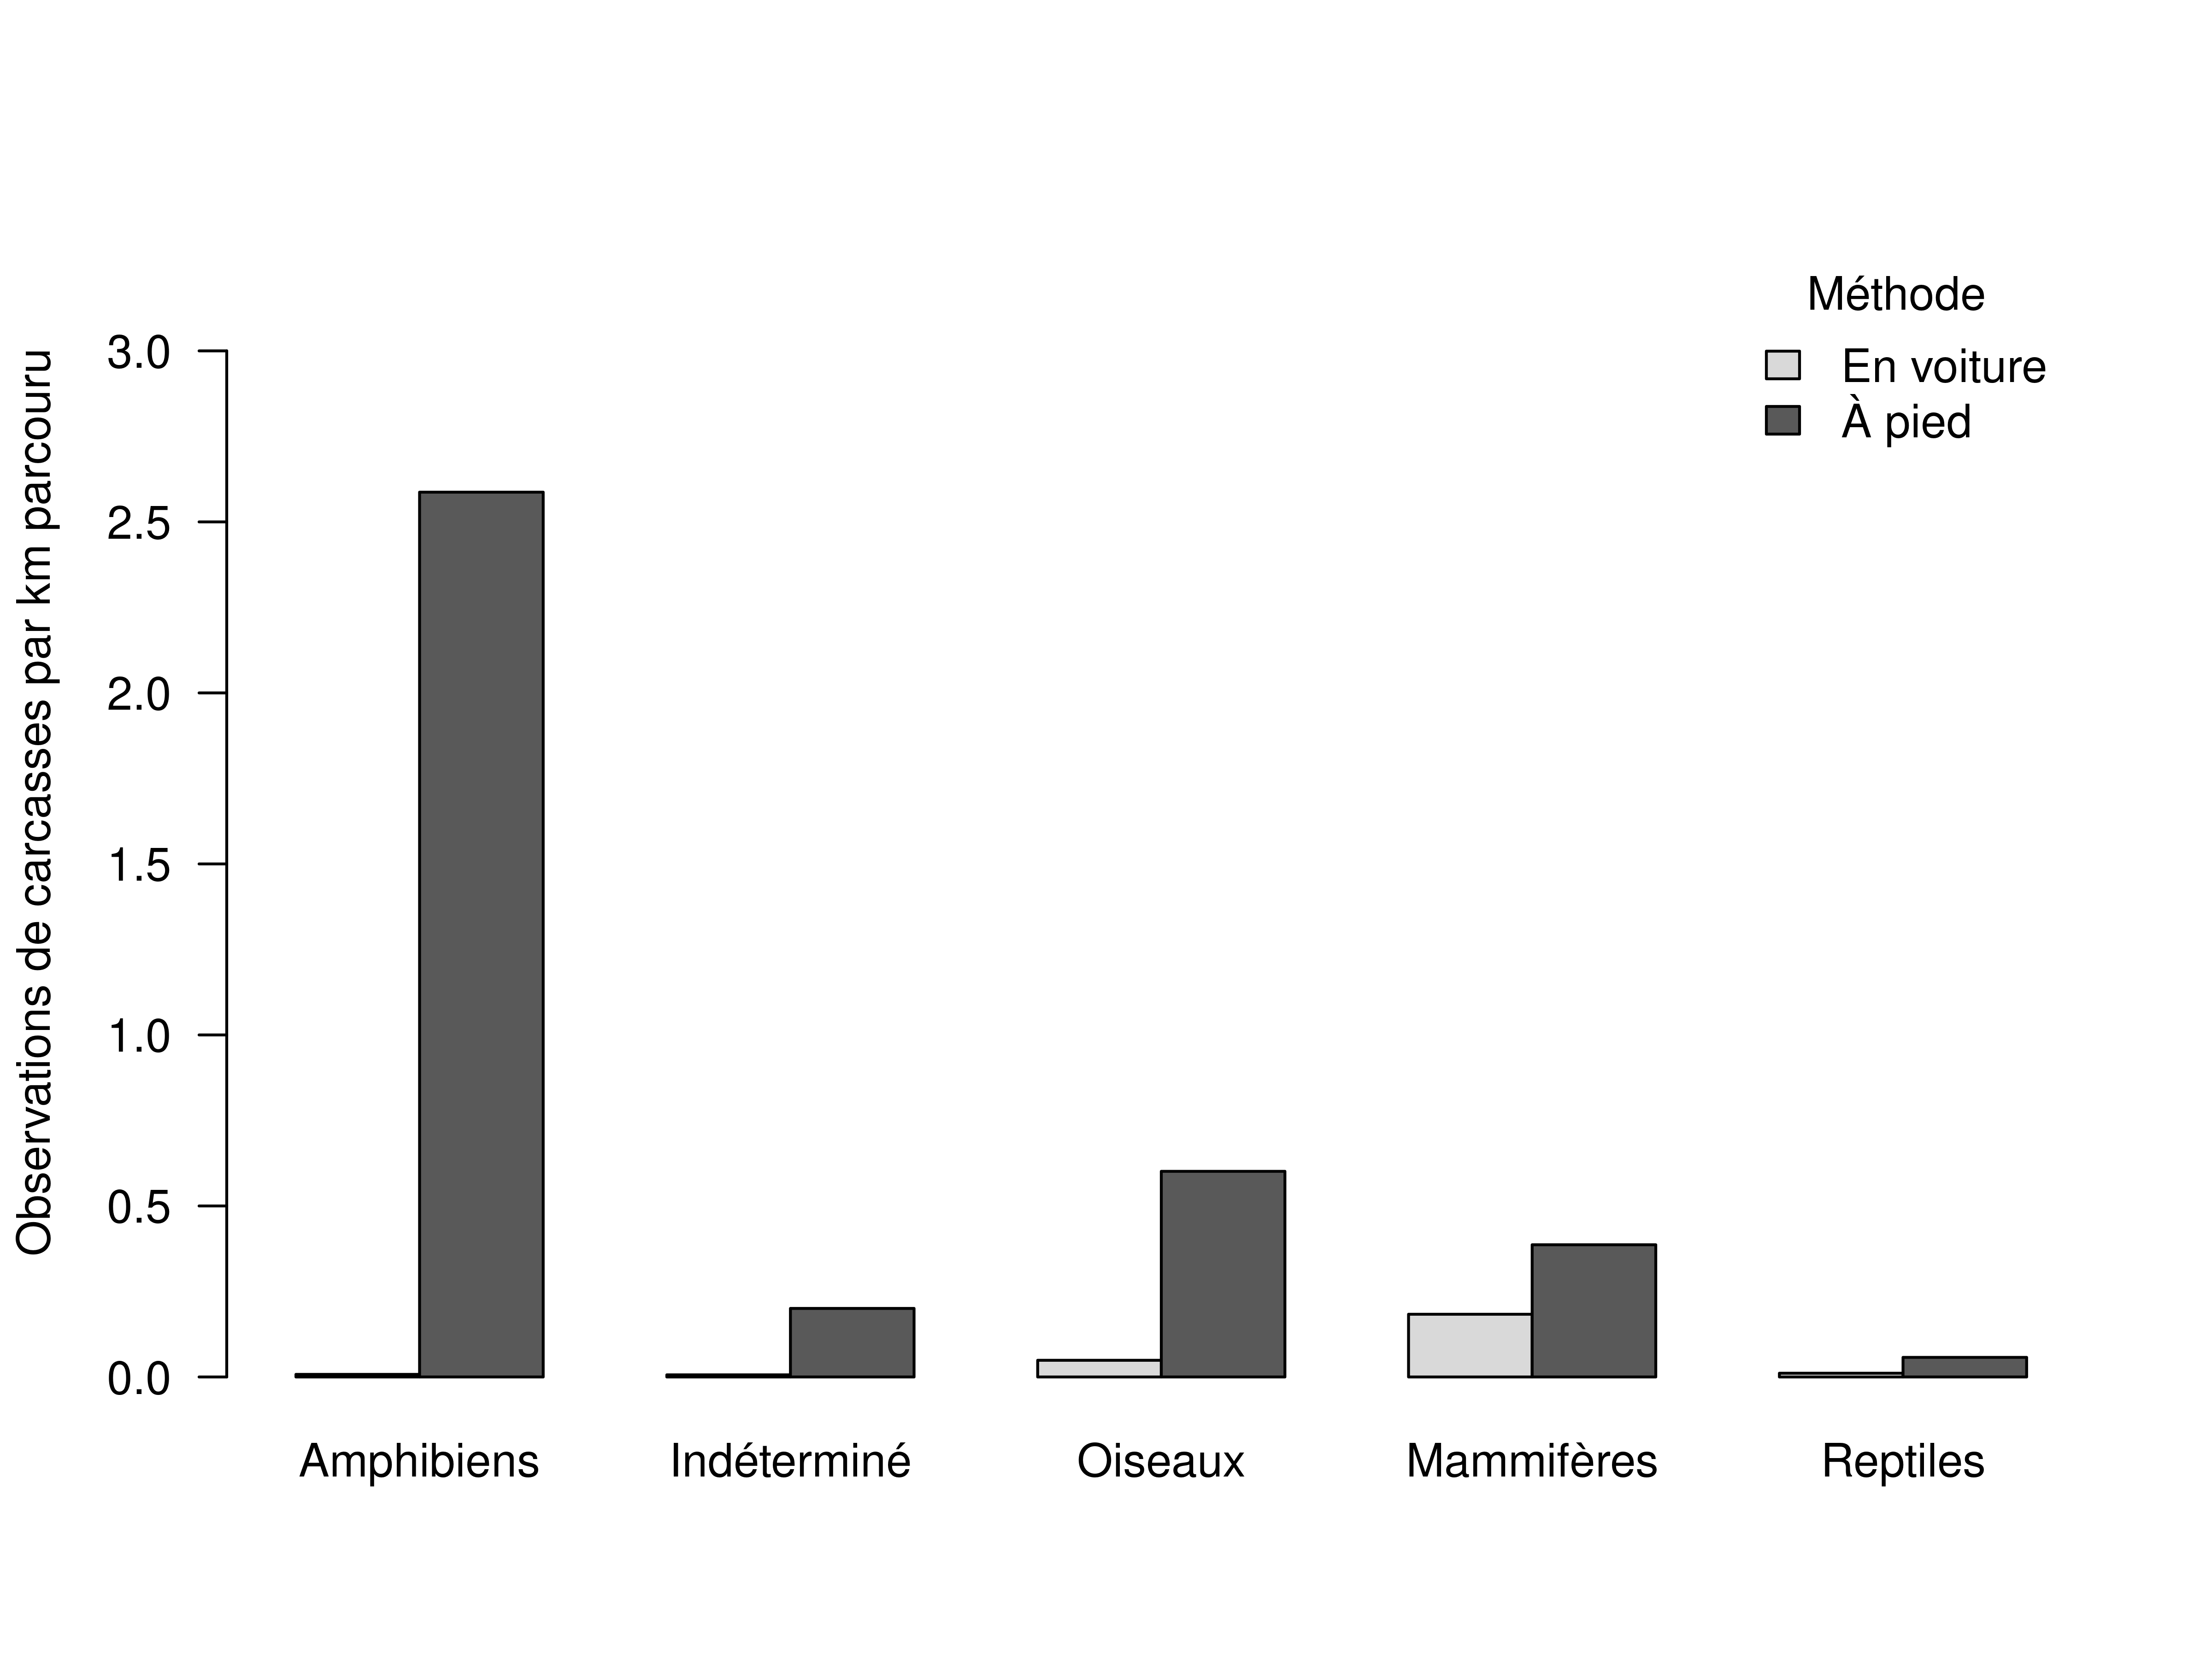
\includegraphics[width=0.8\textwidth]{figs_monteregie_liv3/morts_pond_2026.png}
\caption{Nombre de carcasses observées ramenées au kilomètre parcouru selon la méthode d'échantillonnage, sur un tronçon de l'A35. Données récoltées lors de 206 inventaires (104 en voiture, 102 à pied) réalisés du 19 mai au 21 août 2026. Les parcours en voiture englobent le tronçon inventorié à pied, mais s'étendent en amont et en aval sur un linéaire plus long avec potentiellement des habitats différents. De ce fait, ces écarts entre les deux méthodes traduisent  à la fois une différence de détectabilité inhérente à la méthode ainsi qu'une différence dans les habitats échantillonnés.}
\label{fig:bar_hor_bino26}
\end{figure}


\subsubsection{Persistance}

Globalement, les tests de persistances révèlent que peu de morceaux de poulet étaient prélevés par des prédateurs , soit seulement 12,3~\%. Dans le livrable précédent il avait déjà été constaté que la persistance apparaissait comme nettement plus faible sur d'autres projet actuellement en cours au Bas-Saint-Laurent ou au Nouveau-Brunswick. Par ailleurs le temps moyen de prédation était également assez long, soit environ 16 h 00.

\subsubsection{Enregistrements acoustiques et suivi des milieux humides}

Pour lLe modèle entraîné pour la grenouille du Nord et la grenouille léopard n'a détecté aucune grenouille du Nord parmi les 12 904 fichiers d'enregistrement de 2025. Il est peu probable que cette absence de détection soit attribuable à une faiblesse du modèle. En effet, les tests réalisés en laboratoire montrent que, malgré un taux élevé de faux positifs, le modèle détecte bien l'espèce lorsqu'elle est présente, et ce, même dans des contextes variés. Par ailleurs, l'absence d'observation de grenouille du Nord lors des inventaires visuels plaide pour une absence de l'espèce sur les sites. En revanche, ce qui paraît davantage surprenant c'est la faible occurence de la grenouille léopard sur l'ensemble des sites suivis. D'autres analyses avec l'outil birdNET seront faites pour le prochain livrable avec un nouveau modèle, entraîtné avec davantage de fichiers, ce qui permettra de valider définitivement ces premiers résultats. 

Initialement, le protocole des inventaires visuels prévoyait le dénombrement des adultes, des juvéniles, des larves et des masses d'\oe{}ufs. En 2025, les décomptes précis de masses d'\oe{}ufs par espèce n'ont pas pu être réalisés, l'identification et le dénombrement des pontes s'étant révélés trop exigeants pour être appliqués de manière fiable sur le terrain, seule la présence ou l'absence de masses d'\oe{}ufs a pu être consignée par les auxiliaires.

La rainette versicolore, espèce la plus fréquemment détectée par l'enregistrement acoustique passif, est celle dont le nombre d'occurrences était le plus faible lors des inventaires visuels. Ce contraste illustre la complémentarité des deux approches. En effet, les espèces de petite taille et avec des m\oe{}urs arboricoles, telles que la rainette versicolore, sont difficiles à localiser dans la végétation. Il est donc attendu que cette espèce soit mieux détectée par les méthodes passives que par la recherche active.

À l'inverse, des espèces de plus grande taille et se trouvant facilement en bordure des étangs se prête mieux à des inventaires visuels. Néanmoins, il est tout de même surprenant que la grenouille verte ne soit pas davantage détectée par l'intermédiaire du dispositif d'enregistrement passif. Il est possible que l'emplacement utilisé pour positionner l'audiomohts ne soit pas optimal pour détecter les espèces sur un endroit. 

Le fait que la grenouille des bois n'ait pas été détecté est potentiellement dû à un début d'échantillonnage trop tardif. 



% Refs
% \nocite{*}
\bibliographystyle{ecologyNewFR}
\bibliography{R875-1}
%add références to table of contents
\addcontentsline{toc}{section}{Références}

%deactivate automatic space after colon in references
\shorthandoff{:}


% print all comments at the end
\listoftodos

\end{document}
